\chapter{Introducción}
\label{seccion_geometria_introduccion}

\section{Puntos, segmentos, marcas de igualdad.}\label{subseccion_puntos_segmentos_etc}
\textit{Que es un Punto?} La mínima marca que deja un lápiz, un pobre solo en la nada.

\begin{figure}[H]
	\centering
	
\includegraphics[width=0.15\linewidth]{Geometria/imgs/punto.png}
%	\caption{}
	\label{punto}
\end{figure}
\textbf{OJO.} Lo debemos nombrar usando \textbf{letras mayúsculas}.

\begin{figure}[H]
	\centering
	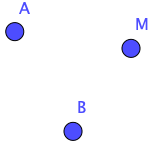
\includegraphics[width=0.15\linewidth]{Geometria/imgs/puntos}
	%	\caption{}
	\label{puntos}
\end{figure}

\textit{Ahora si tenemos dos puntos, cómo hacemos para llegar de uno al otro?}

\begin{figure}[H]
	\centering
	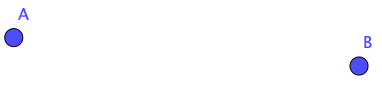
\includegraphics[width=0.4\linewidth]{Geometria/imgs/puntos_A_y_B}
	%	\caption{}
	\label{puntos_A_y_B}
\end{figure}

\textbf{Rta:} Podriamos con muchos caminos, \textit{como cuales?}. De estos \textit{cuál es el más corto?} \textbf{Rta:} El \textbf{segmento}.

\begin{figure}[H]
	\centering
	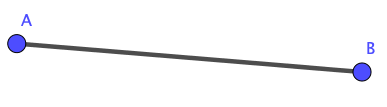
\includegraphics[width=0.5\linewidth]{Geometria/imgs/segmento_AB}
	\caption{Segmento $\overline{AB}$}
	\label{segmento_AB}
\end{figure}

\textbf{OJO.} Un \textbf{segmento} se denota por sus puntos extremos, en este caso el de la figura \ref{segmento_AB} se denota como \textbf{segmento $\overline{AB}$ }. A veces para referirnos a la longitud simplemente decimos $AB=12cm$. 


\rule{\textwidth}{0.1mm}
\begin{act}
	Construir en geogebra un lado $AB$ y luego construir otro lado $CD$ que sea el triple que este (Mejor si logra crear un deslizador para el valor de la razón incluso si logra crear un deslizador).
\end{act}
\rule{\textwidth}{0.1mm}

\textit{Cúantos puntos tiene un segmento? } \textbf{Rta:} Infinitos.

\begin{figure}[H]
	\centering
	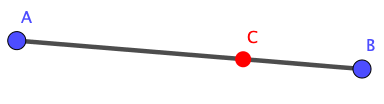
\includegraphics[width=0.4\linewidth]{Geometria/imgs/punto_C_sobre_AB}
	\caption{Un punto $C$ sobre $\overline{AB}$}
	\label{punto_C_sobre_AB}
\end{figure}

\begin{figure}[H]
	\centering
	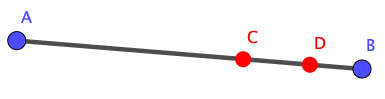
\includegraphics[width=0.4\linewidth]{Geometria/imgs/puntos_C_D_sobre_AB}
	\caption{Dos puntos, $C$ y $D$ sobre $\overline{AB}$}
	\label{puntos_C_D_sobre_AB}
\end{figure}

\textit{Entre un par de puntos en un segmento siempre encontrará otro punto?} \textbf{Rta:} Si.

\rule{\textwidth}{0.1mm}
\begin{act}
	Construir en geogebra un segmento $\overline{AB}$ e ir poniendo puntos y haciendo zoom para ver que siempre entre cada par de puntos habrá otro.
\end{act}
\rule{\textwidth}{0.1mm}

\textbf{OJO.} Leer lo siguiente a ver que se entiende, es un ejercicio útil a la hora de resolver problemas, identificar palabra por palabra.\\
\textit{Cuántos puntos \textbf{equidistantes} a $A$ y $B$ hay en un segmento $\overline{AB}$?} \textbf{Rta:} Es decir punto $X$ tal que $AX=XB$, hay uno ver figura \ref{punto_medio}.
 
\begin{figure}[H]
	\centering
	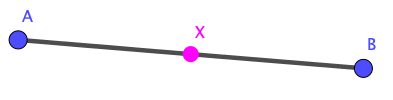
\includegraphics[width=0.5\linewidth]{Geometria/imgs/punto_medio}
	\caption{Punto medio  $X$ de $\overline{AB}$, es decir, $AX=XB$}
	\label{punto_medio}
\end{figure}

Para denotar longitudes iguales se usan marcas, ejemplos:

\begin{figure}[H]
	\centering
	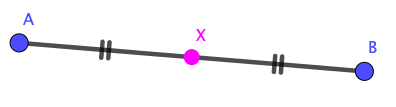
\includegraphics[width=0.5\linewidth]{Geometria/imgs/notacion_longitud_igual}
	\caption{$AX=XB$}
	\label{notacion_longitud_igual}
\end{figure}

\begin{figure}[H]
	\centering
	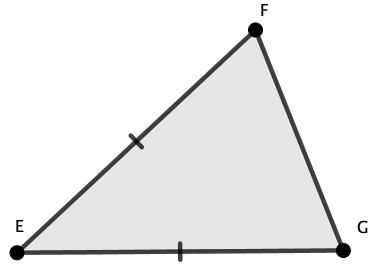
\includegraphics[width=0.5\linewidth]{Geometria/imgs/notacion_en_un_triangulo}
	\label{notacion_en_un_triangulo}
\end{figure}


\begin{exer}{\ \\}
		Si no fuera sobre el segmento, habrán mas puntos equidistantes a $A$ y $B$?
\end{exer}

\newpage
\begin{center}
		\vspace{-1cm}
		\subsection{ Puntos, segmentos, marcas de igualdad.}\label{ejercicios_puntos_segmentos_etc} 
\end{center}
			
\begin{enumerate} 
	\item  En la figura \ref{notacion_longitud_igual} se tiene que $AB=10cm$, entonces cuánto mide $AX$?
	\item\label{ejer_problema_segmento_dividido_en_tres} En la figura \ref{problema_segmento_dividido_en_tres} se tiene que $HK=12cm$, entonces cuánto mide $IJ$?
		
		\begin{figure}[H]
			\centering
			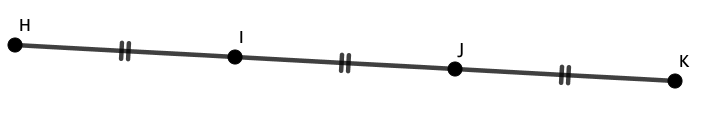
\includegraphics[width=0.8\linewidth]{Geometria/imgs/problema_segmento_dividido_en_tres}
			\caption{Ejercicio \ref{ejer_problema_segmento_dividido_en_tres}.}
			\label{problema_segmento_dividido_en_tres}
		\end{figure}
	\item \label{ejer_problema_2} En la figura \ref{problema_2} se tiene que $AB=12cm$, si $AX = XB$ y $AL=LX$ entonces cuánto mide $LB$?
		
		\begin{figure}[H]
			\centering
			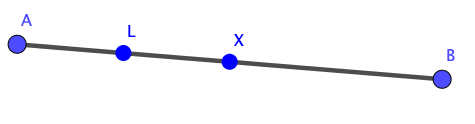
\includegraphics[width=0.8\linewidth]{Geometria/imgs/problema_2}
			\caption{Ejercicio \ref{ejer_problema_2}.}
			\label{problema_2}
		\end{figure}
	
	\item \label{ejer_problema_3} En la figura \ref{problema_3} se tiene que $NO=12cm$, si $OB=4cm$ y $AX=3cm$ entonces cuánto es el perimetro de $NOBA$?
	
	\begin{figure}[H]
		\centering
		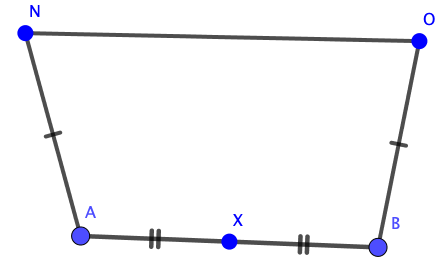
\includegraphics[width=0.6\linewidth]{Geometria/imgs/problema_3}
		\caption{Ejercicio \ref{ejer_problema_3}.}
		\label{problema_3}
	\end{figure}		
\end{enumerate}
\newpage

\section{Rectas, rayo, paralelas, rectas concurrentes}\label{subseccion_rayo_recta_paralelas_etc}

Sabiamos que con un segmento podíamos ir de un punto a otro, ahora seguiremos derecho al pasar por un punto hasta donde queramos mediante el \textbf{rayo}.

\begin{figure}[H]
	\centering
	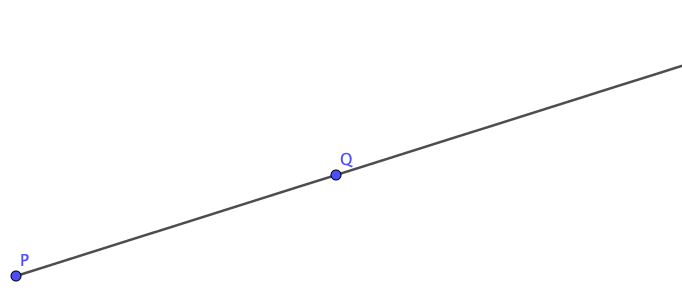
\includegraphics[width=0.8\linewidth]{Geometria/imgs/rayo}
	\caption{Un \textbf{rayo} $\overset\rightarrow{PQ}$ que parte de $P$ y pasa por $Q$.}
	\label{rayo}
\end{figure}

\textbf{OJO. } Al \textbf{rayo} que parte de $P$ y pasa por $Q$ se le denota como $\overrightarrow{PQ}$.\\

\textit{Será que $\overrightarrow{PQ}$ es lo mismo que $\overrightarrow{QP}$?} \textbf{Rta:} No.\\
\textit{Coloquen un punto que esté en  $\overrightarrow{PQ}$ y no esté en  $\overrightarrow{QP}$ }\\
\textit{Coloquen un punto que esté en  $\overrightarrow{PQ}$ y en  $\overrightarrow{QP}$ }\\
\textit{Coloquen un punto que esté en  $\overrightarrow{QP}$ y no esté en  $\overrightarrow{PQ}$ }.\\

Si ahora seguimos derecho al pasar por ambos puntos hasta donde queramos obtenemos una \textbf{recta}.
\begin{figure}[H]
	\centering
	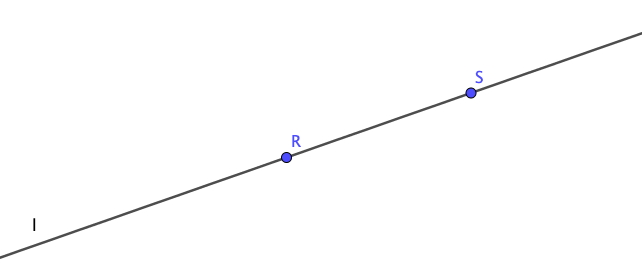
\includegraphics[width=0.8\linewidth]{Geometria/imgs/recta}
	\caption{Una \textbf{recta} $\overset\leftrightarrow{RS}$ o $l$ que pasa por $R$ y $S$.}
	\label{recta}
\end{figure}

\textbf{OJO. } A la \textbf{recta} que que pasa por $R$ y $S$ se le denota como $\overleftrightarrow{RS}$ o se le llama con una letra minúscula ejemplo: $l$.\\

\textit{Si se trazan dos rectas en cuántos puntos se pueden cortar?} \textbf{Rta: }Puede ser en 0 punto como en la figura \ref{paralelas}

\begin{figure}[H]
	\centering
	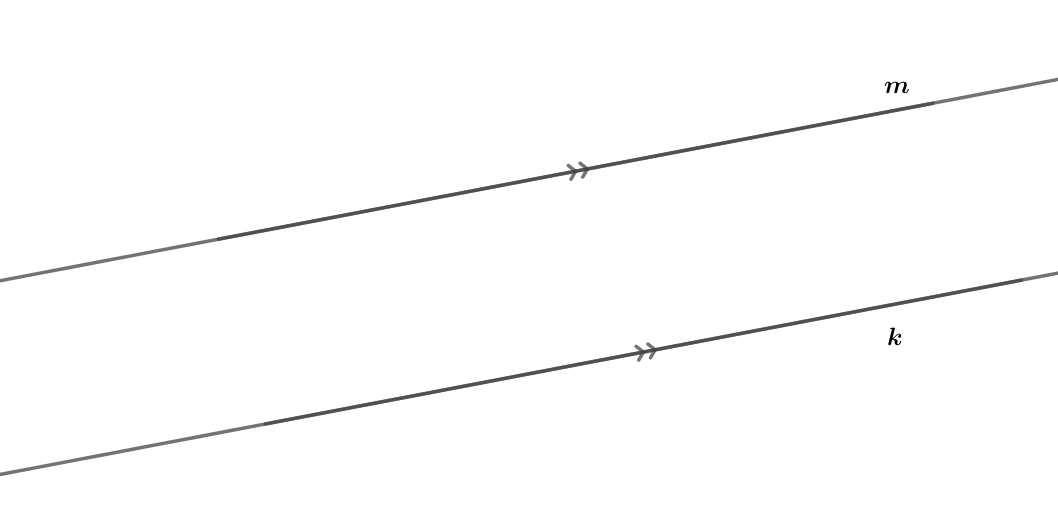
\includegraphics[width=0.7\linewidth]{Geometria/imgs/paralelas}
	\caption{Las rectas $k$ y $l$ son paralelas o sea $l||k$.}
	\label{paralelas}
\end{figure}

\textbf{OJO. }Un par de rectas $k$ y $l$ son \textbf{paralelas} si nunca se cortan, esto se denota como $l||k$ .\\

\textbf{Rta: }Puede ser en 1 punto como en la figura \ref{concurrentes}

\begin{figure}[H]
	\centering
	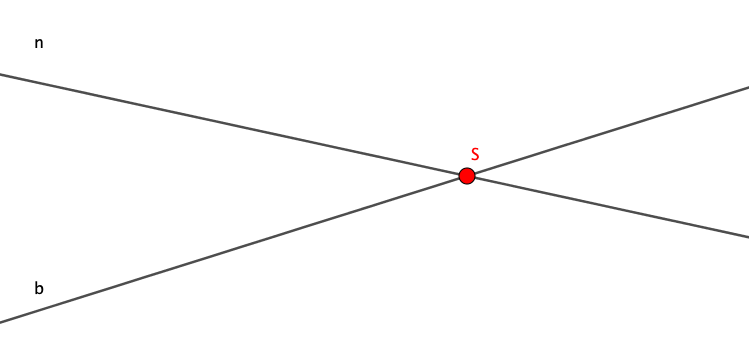
\includegraphics[width=0.85\linewidth]{Geometria/imgs/concurrentes}
	\caption{Las rectas $n$ y $b$ son concurrentes o se intersectan en $S$.}
	\label{concurrentes}
\end{figure}

\textbf{OJO. }Un par de rectas $n$ y $n$ son \textbf{concurrentes} o se \textbf{intersectan} si comparten 1 punto.\\

\textit{Será que dos rectas se pueden intersectar en 2 puntos ?}

\textbf{OJO.} Si varios puntos están sobre una misma recta se dice que son \textbf{colineales}, ver figura \ref{colineales}.

\begin{figure}[H]
	\centering
	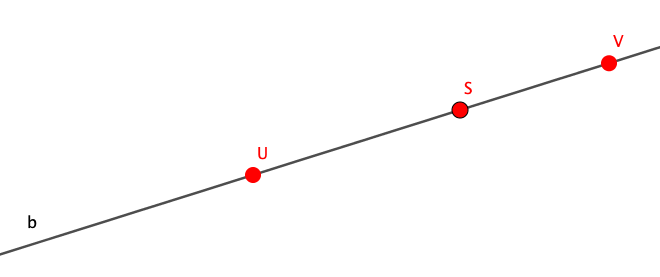
\includegraphics[width=0.85\linewidth]{Geometria/imgs/colineales}
	\caption{Los puntos $U$, $S$ y $V$ son colineales pues están todos sobre la recta $b$.}
	\label{colineales}
\end{figure}

\textit{Es diferente la recta $\overleftrightarrow{US}$ que $\overleftrightarrow{VS}$ ?}\\

\newpage
\begin{center}
	\vspace{-1cm}
	\subsection{Ejercicios: Rectas, rayo, paralelas, rectas concurrentes.}\label{ejercicios_subseccion_rayo_recta_paralelas_etc}
\end{center}
	\begin{enumerate}
		\item Realizar los puntos del 1. al 9.
		\begin{figure}[H]
			\centering
			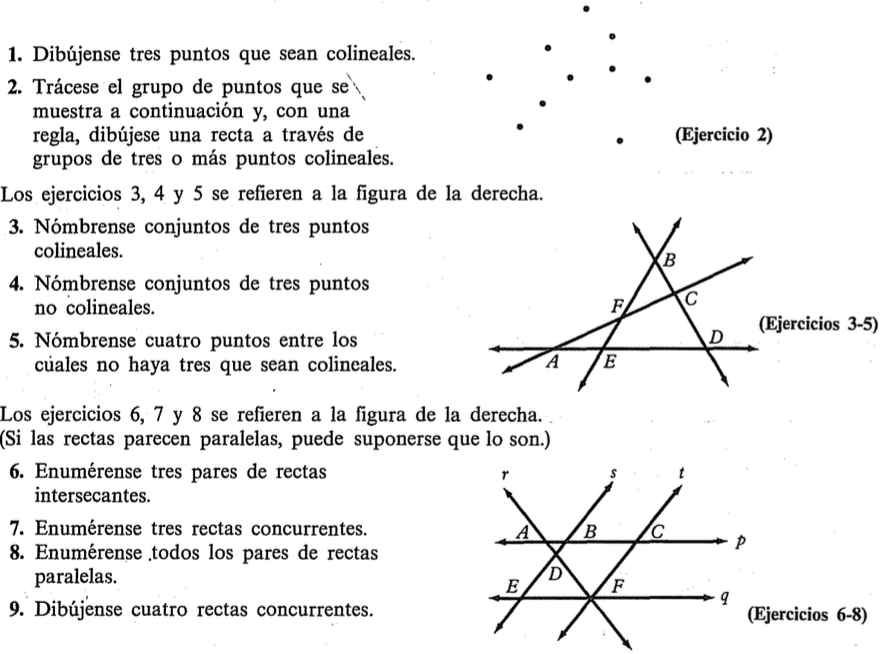
\includegraphics[width=\linewidth]{Geometria/imgs/Clemens_p14_1to9}
			%\caption{Los puntos $U$, $S$ y $V$ son colineales pues están todos sobre la recta $b$.}
			\label{Clemens_p14_1to9}
		\end{figure}
		\item Realizar los puntos del 12. al 14.
		\begin{figure}[H]
			\centering
			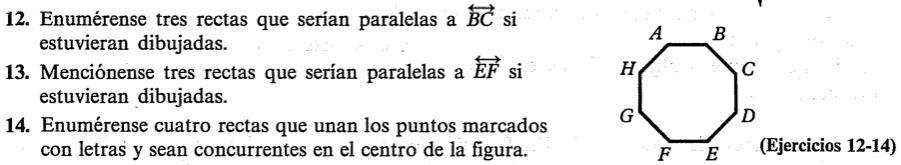
\includegraphics[width=\linewidth]{Geometria/imgs/CLEMENS_p15_12to14}
			%\caption{Los puntos $U$, $S$ y $V$ son colineales pues están todos sobre la recta $b$.}
			\label{CLEMENS_p15_12to14}
		\end{figure}
		\item (1.2.1 de \cite{Aops_Geometria}). Alicia está pensando en una recta. Cuántos puntos en esta recta le debe mostrar a Bernardo para que el sepa en que recta está pensando ella?
		\item (1.2.2 de \cite{Aops_Geometria}). $M$ es el punto medio de $\overline{AB}$ y $N$ es el punto medio de $\overline{BM}$. Si $BN=4cm$, cuánto mide $AB$?
		\item (1.2.3 de \cite{Aops_Geometria}). $P,Q,R,S$ y $T$ están en una recta $k$ tal que $Q$ es el punto medio de $\overline{PT}$, $R$ es el punto medio de $\overline{QT}$  y $S$ es el punto medio de $\overline{RT}$. Si $PS=9cm$, cuánto mide $PT$?
		\item (1.2.4 de \cite{Aops_Geometria}). \textbf{(Woww)}. Los puntos $A,B,C,D$ y $E$ están sobre el segmento que tiene como puntos finales a $A$ y $E$. Los puntos están en el orden que fueron mencionados de izquierda a derecha de forma que $CD=\frac{AB}{2}$, $BC=\frac{CD}{2}$, $AB=\frac{AE}{2}$ y $AE=12cm$. Cuánto mide $AD$?		
	\end{enumerate}
\newpage

\section{Circulo, radio, tangente, secante, cuerda, diámetro, arco}\label{subseccion_de_introduccion_geo_circulo}

\rule{\textwidth}{0.1mm}
\begin{act_clase} \textbf{En el circulo}\\ (\textit{Basado en \cite{Aops_Geometria} problemas 1.1 y 1.2}){\ \\}
	
	\textbf{Materiales:} 
	\begin{enumerate}
		\item Regla.
		\item Compás.
		\item Lápiz.
	\end{enumerate}

	\textbf{Desarrollo:}
	\begin{enumerate}
		\item Marcar un punto $O$, luego con el solo uso de la regla encontrar la mayor cantidad de puntos que estén a 2cm de $O$, nombrar estos puntos $A,B,C,D,\dots$ y así sucesivamente. Si se dibujan muchos de estos puntos que figura se forma?
		\vspace{6cm}
		
		\begin{itemize}
			\item Esto es un \textbf{circulo}, donde $O$ es el \textbf{centro del círculo}. En vez de decir \textit{``circulo con centro en $O$""} se puede decir: $\odot O$. 
			\item El segmento \textbf{$\overline{AB}$ es un radio} de $\odot O$. Mencione otros radios de $\odot O$: \vspace{1cm}
			
			\item La distancia del centro $O$ a los puntos también se conoce como radio, es decir \textbf{el radio del $\odot O$ es de 2cm} .
		\end{itemize}
		
		
		\item Dado $\odot X$ de radio $1.5cm$ trazar:
		\begin{enumerate}[label=\Alph*)]
				\item Una recta $l$ que corte al circulo en cero puntos. \vspace{5cm}
				\item Una recta $k$ que corte al circulo en 1 punto. \vspace{5cm}
						\begin{itemize}
							\item Esta recta que solo toca en 1 punto al circulo recibe el nombre de: \textbf{recta tangente}. Se dice entonces que $l$ es tangente a $\odot X$.
						\end{itemize}
				\item Una recta $m$ que corte al circulo en 2 puntos. \vspace{5cm}
						\begin{itemize}
							\item Esta recta que intersecta en 2 puntos al circulo recibe el nombre de: \textbf{recta secante}. Se dice entonces que $m$ es secante a $\odot X$.
						\end{itemize}
				\item Habrá una recta que corte en 3 puntos al circulo?
		\end{enumerate}
		\item Dibujar un $\odot O$ de radio $2cm$ y un recta $m$ que sea tangente a $\odot O$ en un punto $P$.\vspace{5cm}
		\item Dibujar un $\odot R$ de radio $1.7cm$ y un recta $s$ que sea secante a $\odot R$ en los puntos $P$ y $Q$. \vspace{5cm}
		
		\item Dado $\odot Y$ de radio $1.2cm$ trazar:
			\begin{enumerate}[label=\Alph*)]
				\item Todas las formas posibles en que un segmento $\overline{RS}$ corte al circulo en cero puntos. \vspace{5cm}
				\item Todas las formas posibles en que un segmento $\overline{PQ}$ corte al circulo en 1 punto. \vspace{5cm}
				\item Todas las formas posibles en que un segmento $\overline{CT}$ corte al circulo en 2 puntos. \vspace{5cm}
				\begin{itemize}
					\item En el caso en el los puntos del segmento están sobre el circulo es especial. Se dice en este caso que el segmento es una \textbf{cuerda}. 
				\end{itemize}
			\end{enumerate}
		\item Dibuje un $\odot M$ de radio $3cm$ y dibuje:
				\begin{enumerate}[label=\Alph*)]
						\item Una cuerda $\overline{AB}$ de forma que $AB=6cm$.
						\item Una cuerda $\overline{RS}$ de forma que $AB=4cm$.
						\item Una cuerda $\overline{PQ}$ de forma que $AB=2cm$.
				\end{enumerate}
		 		\vspace{8cm}
		 \item Qué diferencia hay entre una cuerda y una secante?\vspace{1.5cm}
		 \item Dado $\odot Q$ de radio cualquiera, construir una cuerda $\overline{XY}$ que pase por $Q$.\vspace{4cm}
			 \begin{enumerate}[label=\Alph*)]
			 		\item Es $Q$ equidistante a $X$ y $Y$? Por qué?\vspace{1.5cm}
			 \end{enumerate}
		 	\begin{itemize}
		 		\item La cuerda que pasa por el centro de un circulo recibe el nombre de \textbf{diámetro}. En el anterior ejemplo tenemos entonces que el diámetro es la cuerda $XY$. Habrán más diámetros? Dibuje mas puntos si es necesario y mencioe acá otros diámetros:\vspace{2cm}
		 		
		 	\end{itemize}
	 	\item Cuántos diámetros tiene un circulo?
	 	\item Trazar $\odot Q$ de forma que los diámetros del circulo midan $4cm$.\vspace{5cm}
	 	\item Trazar $\odot N$ de radio $1.5cm$ y dos puntos $A$ y $H$ sobre el circulo. Luego trazar la curva más corta que une a $A$ y $H$ sobre el circulo.\vspace{4cm}
	 	\begin{itemize}
	 		\item La curva que une a $A$ y $H$ es un \textbf{arco}. Es la curva mas corta que une dos puntos sobre el circulo.
	 	\end{itemize}
	\end{enumerate}
\end{act_clase}
\rule{\textwidth}{0.1mm}

\newpage
\begin{center}
	\vspace{-1cm}
	\subsection{Ejercicios: Circulo, radio, tangente, secante, cuerda, diámetro, arco}\label{ejercicios_subseccion_de_introduccion_geo_circulo}
\end{center}
	\begin{enumerate}				
			\item \label{p131_aops_geo} (1.3.1 de \cite{Aops_Geometria}). En la Figrua \ref{aops_geo_p_1_3_1} identifique cuando cada uno de los siguientes es una secante, una recta, una cuerda, un radio, un diámetro o una recta tangente a $\odot O$. (Si cumple con varios terminos, mencionelos todos):
			\begin{enumerate}[label=\Alph*)]
					\item $\overline{CO}$.
					\item $\overleftrightarrow{EF}$.
					\item $\overline{CD}$.
					\item $\overline{AB}$.
					\item $\overleftrightarrow{CD}$.
			\end{enumerate}
			
				\begin{figure}[H]
					\centering
					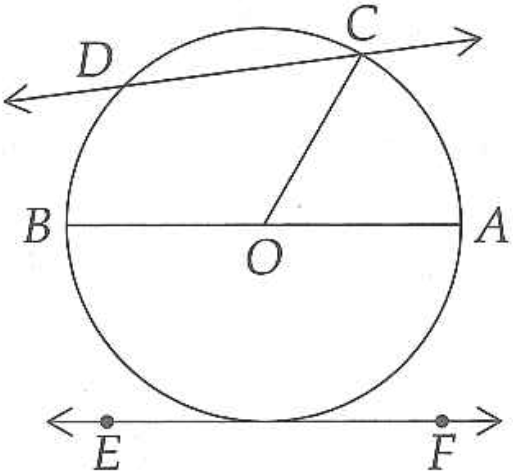
\includegraphics[width=0.35\linewidth]{Geometria/imgs/aops_geo_p_1_3_1}
					\caption{Ejercicio \ref{p131_aops_geo}}
					\label{aops_geo_p_1_3_1}
				\end{figure}
			\item \label{p132_aops_geo} (1.3.2 de \cite{Aops_Geometria}). Suponga que tiene un punto $P$ fuera de un circulo cualquiera. Siempre es posible trazar una recta que pase por $P$ y sea tangente al circulo?
			
			\item \label{p133_aops_geo} (1.3.3 de \cite{Aops_Geometria}). Cuánto es la máxima cantidad posible que puede haber de puntos de intersección entre un cirulo y un triángulo?
			
			\item \label{p134_aops_geo} (1.3.4 de \cite{Aops_Geometria}). \textbf{Wow}. Se tienen dos circulos y tres rectas sobre el mismo plano. Cuánto es la máxima cantidad posible que puede haber de puntos de intersección donde al menos dos figuras se intersectan?
	\end{enumerate}
\newpage

\section{Copiando segementos}\label{Copiando_segmentos}
\rule{\textwidth}{0.1mm}
\begin{act_clase} \textbf{Copiando segmentos} \\ (\textit{Basado en \cite{Aops_Geometria} problemas 1.3 y 1.4}){\ \\}
	\textbf{Materiales:} 
	\begin{itemize}
		\item Regla.
		\item Compás.
		\item Lápiz.
		\item Transportador.
	\end{itemize}
	
	\textbf{Desarrollo:} De acá en adelante no se puede usar la regla para medir!
	\begin{enumerate}
		\item Dados dos puntos $A$ y $B$ donde quieran, trazar un $\odot A$ que pase por $B$ y se llame $c_1$ y otro $\odot B$ que pase por $A$ y se llame $c_2$. \vspace{8cm}
		
		\begin{itemize}
				\item \textbf{Dato:} Al igual que las rectas, también podemos llamar a los circulos con letras minúsculas.
		\end{itemize}
	
		\item Trazar un segmento $\overline{AB}$ de longitud aleatoria, luego hacer un circulo $\odot M$ cuyo radio sea $\overline{AB}$
		\vspace{6cm}
		
		\item (1.3 de \cite{Aops_Geometria}). Usar el compás para hallar en la recta $k$ un punto $Y$ tal que $AB=XY$.
			\begin{figure}[H]
				\centering
				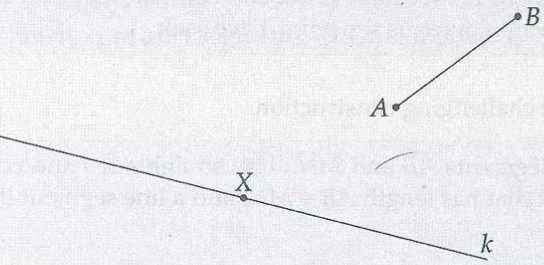
\includegraphics[width=0.8\linewidth]{Geometria/imgs/aops_geo_1_3}
				%\caption{}
				\label{aops_geo_1_3}
			\end{figure}

		\item \label{p1_4_aopsgeo}(1.4 de \cite{Aops_Geometria}). En la figura \ref{aops_geo_1_3} se muestran los segmentos $\overline{AB}$ y $\overline{MN}$. Con regla y compás construir:
			\begin{figure}[H]
				\centering
				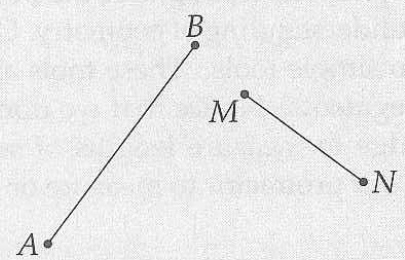
\includegraphics[width=0.5\linewidth]{Geometria/imgs/aops_geo_1_4}
				\caption{Ejercicio \ref{p1_4_aopsgeo}}
				\label{aops_geo_1_4}
			\end{figure}
		\begin{enumerate}[label=\Alph*)]
				\item Un segmento de longitud $AB+MN$. \vspace{6cm}
				\item Un segmento de longitud $AB-MN$. \vspace{7cm}
				\item Un segmento de longitud $MN-AB$. \vspace{7cm}				
		\end{enumerate}

		\item \label{p1_4_1_aopsgeo} (1.4.1 de \cite{Aops_Geometria}). Con los segmentos de la figura \ref{aops_geo_1_4_1}, construir:
			\begin{figure}[H]
				\centering
				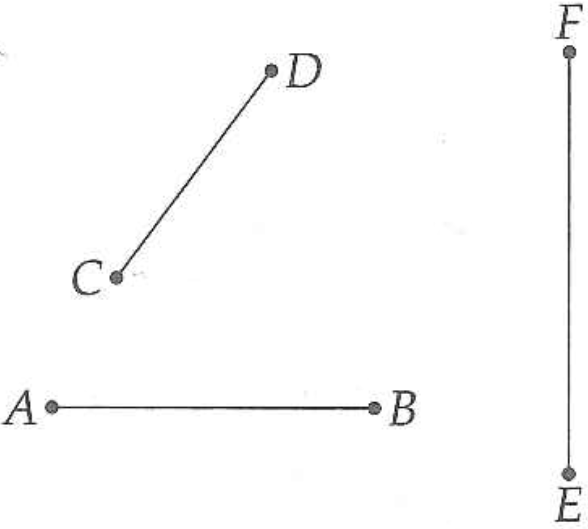
\includegraphics[width=0.3\linewidth]{Geometria/imgs/aops_geo_1_4_1}
				\caption{Ejercicio \ref{p1_4_1_aopsgeo}}
				\label{aops_geo_1_4_1}
			\end{figure}
			\begin{enumerate}[label=\Alph*)]
				\item Un segmento de longitud $AB+CD-EF$. \vspace{6cm}
				\item Un segmento de longitud $2AB$. \vspace{6cm}
				\item Un segmento de longitud $AB-2EF+3CD$. \vspace{5cm}				
			\end{enumerate}
		
	\end{enumerate}
\end{act_clase}
\rule{\textwidth}{0.1mm}
\newpage

\section{Ángulos}\label{subseccion_angulos_intro}

\subsection{Introducción, notacion, clasificacion, medicion.}\label{subsection_intro_notacion_clasificacion_medicion}

\begin{itemize}
	\item Cuando dos rayos comparten el origen forman un \textbf{ángulo}. Este vértice se llama \textbf{vértice del ángulo}. 
	\item Por ejemplo en le Figura \ref{Angulo_XOY} se presenta un ángulo formado por los rayos $\overrightarrow{OX}$ y $\overrightarrow{OY}$, el cuál se denota como $\angle XOY$, \textbf{se nombre el vértice en la mitad}, también se puede llamar $\angle YOX$ \textbf{Ojo:} Pero no $\angle YXO$ ni  $\angle XYO$.
	\item En este caso como solo está este ángulo también se puede denotar como $\angle O$.
\end{itemize}


\begin{figure}[H]
	\centering
	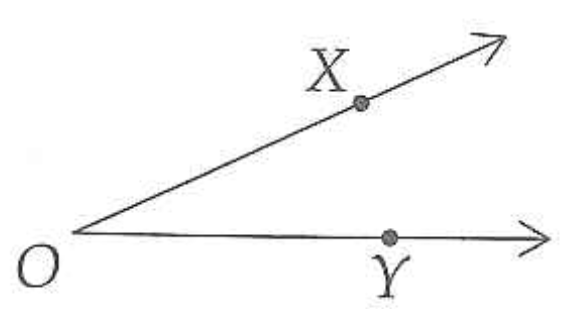
\includegraphics[width=0.3\linewidth]{Geometria/imgs/Angulo_XOY}
	%\caption{Ángulo $\angle XOY$, también puede ser llamado $\angle YOX$}
	\label{Angulo_XOY}
\end{figure}

\textit{Si $\overleftrightarrow{AB}$ y $\overleftrightarrow{CD}$ se intersectan en un punto $P$ como muestra la Figura \ref{dos_angulos}, es claro a cuál ángulo nos referimos si decimos simplemente $\angle P$?}


\begin{figure}[H]
	\centering
	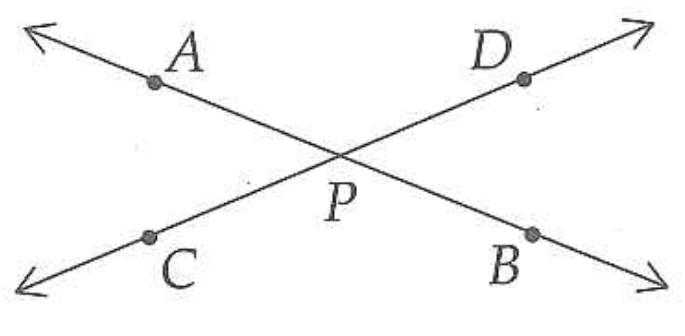
\includegraphics[width=0.3\linewidth]{Geometria/imgs/dos_angulos}
	%\caption{No es correcto decir solo \(\angle P\)}.
	\label{dos_angulos}
\end{figure}

\textbf{Uso de transportador}. Saben usarlo?


\clearpage

%\rule{\textwidth}{0.1mm}

\begin{center}
	$\textbf{\textit{Actividad de clase}}$
\end{center}

\textit{Basado en \cite{Aops_Geometria} problemas 2.1 a 2.5}

\textbf{Materiales:} 
\begin{itemize}
	\item Regla.
	\item Lápiz.
	\item Transportador.
\end{itemize}

\textbf{Desarrollo:}
\begin{enumerate}
	\item Dibujar 3 ángulos abajo, luego intercambiar con otro compa?ero y medir los ángulos que el dibujó. Preguntale si mediste el ángulo que el dibujó.\vspace{6cm}
	\item Cuánto mide el ángulo mas grande que se puede dibujar? Dibujalo. \vspace{5cm}
	\item \label{p22_aops_geo} (2.2 de \cite{Aops_Geometria}). En la Figura \ref{P22_AOPS_GEO} se muestran cuatro ángulos. En cada caso, el punto $O$ es el centro del circulo. $\angle AOB$ corta $\frac{1}{4}$ del circulo,  $\angle COD$ corta $\frac{1}{3}$, $\angle EOF$ corta $\frac{1}{12}$ y $\angle GOH$ corta $\frac{1}{8}$.
	\begin{figure}[H]
		\centering
		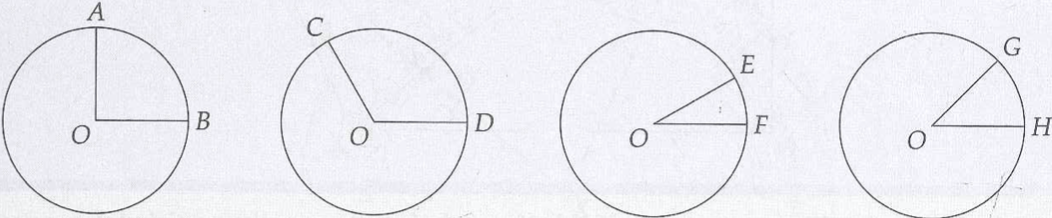
\includegraphics[width=0.75\linewidth]{Geometria/imgs/P22_AOPS_GEO}
		\caption{Punto \ref{p22_aops_geo}}
		\label{P22_AOPS_GEO}
	\end{figure}
	
	\begin{enumerate}[label=\Alph*)]
		\item Cuántos grados mide el ángulo $\angle AOB$?
		\item Cuántos grados mide el ángulo $\angle COD$?
		\item Cuántos grados mide el ángulo $\angle EOF$?
		\item Cuántos grados mide el ángulo $\angle GOH$?		
	\end{enumerate}
	
	\item \label{p23_aops_geo} (2.3 de \cite{Aops_Geometria}). En la Figura \ref{P23_AOPS_GEO} se tiene que $\angle WOY=60\degree$ y $\angle WOX=20\degree$, cuánto mide $\angle XOY$?
	\begin{figure}[H]
		\centering
		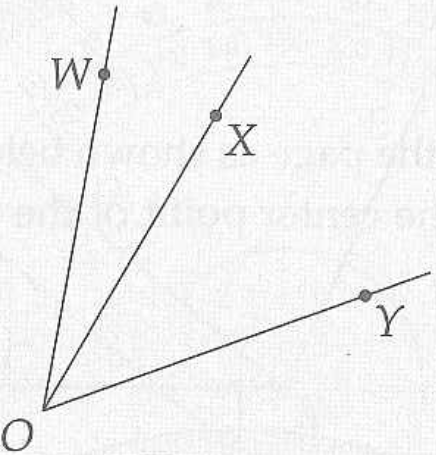
\includegraphics[width=0.3\linewidth]{Geometria/imgs/P23_AOPS_GEO}
		\caption{Punto \ref{p23_aops_geo}.}
		\label{P23_AOPS_GEO}
	\end{figure}
	
	\item \label{P_suma_ang_1}En la Figura \ref{suma_ang_1} se tiene ahora que $\angle WOX=15\degree$ y $\angle XOY=55\degree$, cuánto mide $\angle WOY$?
	\begin{figure}[H]
		\centering
		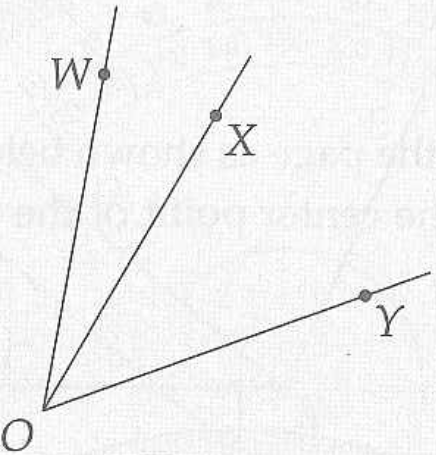
\includegraphics[width=0.3\linewidth]{Geometria/imgs/P23_AOPS_GEO}
		\caption{Punto \ref{P_suma_ang_1}.}
		\label{suma_ang_1}
	\end{figure}
	
	\item \label{ej_8_1_medidaangulos} (Ejemplo 8.1 de \cite{Udea_geometria}) Si se tienen dos ángulos $\angle \alpha$ y $\angle \beta$ que miden $42\degree$ y $35\degree $ respectivamente, cuánto mide $\alpha + \beta$?
	
	
	\item \label{p24_aops_geo} (2.3 de \cite{Aops_Geometria}). Suponga que se mide un ángulo \textit{``interior"}. Como se ve en la figura \ref{P24_AOPS_GEO}, va a haber un ángulo \textit{``exterior"}. Si el ángulo interior $\angle PQR$ mide $40 \degree$, cuánto va a medir el ángulo exterior?
	\begin{figure}[H]
		\centering
		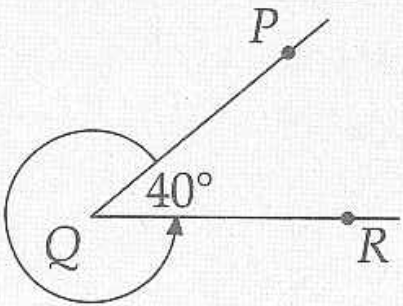
\includegraphics[width=0.3\linewidth]{Geometria/imgs/P24_AOPS_GEO}
		\caption{Punto \ref{p24_aops_geo}.}
		\label{P24_AOPS_GEO}
	\end{figure}
	
	\item Usando 4 rayos, construir un ángulo de $37\degree$ y otro de $143\degree $.\vspace{5cm}
	
	\item Usando 3 rayos, construir un ángulo de $37\degree$ y otro de $143\degree $.\vspace{5cm}
	\begin{itemize}
		\item Al ángulo de $90\degree$ se le conoce como ángulo \textbf{recto}, al de $180\degree$ se le conoce como ángulo \textbf{llano} y al de $360\degree$ se le conoce como ángulo \textbf{completo}.
		\item Cuando un ángulo mide menos de $90\degree $ es un ángulo \textbf{águdo}, cuando mas de $90\degree $ es un ángulo \textbf{obtuso}.
	\end{itemize}
	\item Construir los siguientes ángulos, clasificarlos y decir si tienen un nombre especial: 
	\begin{enumerate}[label=\Alph*)]
		\item $90\degree $. \vspace{4cm}
		\item $45\degree $. \vspace{4cm}
		\item $135\degree $. \vspace{4cm}
		\item $220\degree $. \vspace{4cm} 
		\item $180\degree $. \vspace{4cm}
		\item $270\degree $. \vspace{4cm}																			
	\end{enumerate}
	
	\item Los rayos $OX$ y $OY$ forman un ángulo de $30\degree$. Construir un ángulo que tenga al rayo $OX$ y que mida el triple que $\angle XOY$. \vspace{5cm}	
	
	\item $LR$ es un rayo que está horizontal y $LS$ es otro rayo tal que los rayos $LR$ y $LS$ forman un ángulo de $ \angle SLR=95 \degree$. Construir el rayo $LM$ de tal forma que $LM$ esté entre $LR$ y $LS$, y además el angulo formado por $LR$ y $LM$ mida $25\degree$. Haz el dibujo y luego responde las pregunas: \vspace{5cm}
	\begin{enumerate}[label=\Alph*)]
		\item Cuánto mide $\angle SLR $?					
		\item Cuánto mide $\angle MLR $?
		\item Cuánto mide $\angle SLM $?																								
	\end{enumerate}
	
	
	
\end{enumerate}

%\rule{\textwidth}{0.1mm}
\newpage


\begin{center}
	\vspace{-1cm}
	\subsubsection{Ejercicios:  Ángulos. Clasificación, opuestos por el vértice, suplementarios, complementarios.}\label{ejercicios_subseccion_angulos_intro}
\end{center}
(Tomado de Pag 22-23 de \cite{clemens}) Realizar los siguientes ejercicios.
\begin{figure}[H]
	\centering
	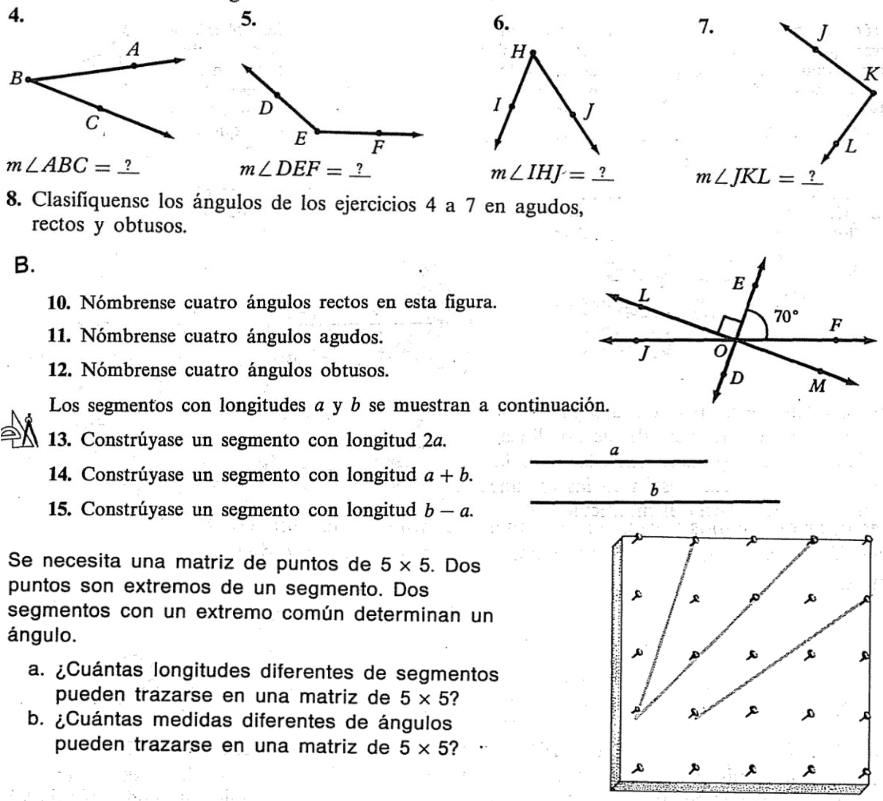
\includegraphics[width=1\linewidth]{Geometria/imgs/ejercicios_clemens_angulos}
	%\caption{}
	%\label{ejercicios_clemens_angulos}
\end{figure}

\newpage

\subsection{Opuestos por el vértice, complementarios, suplementarios.} \label{subsection_opuestosvertices_complementarios_suplementarios}

\begin{ejemplo}
	\label{aopsg_p2_6}
	(2.6 de \cite{Aops_Geometria}). En la figura \ref{aopsgeo_p2_6}, $AOB$ es una linea recta. Cuánto mide el ángulo $\angle AOB$?
	
	\begin{figure}[H]
		\centering
		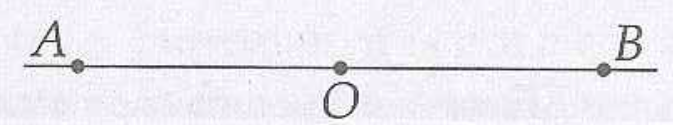
\includegraphics[width=0.7\linewidth]{Geometria/imgs/aopsgeo_p2_6}
		\caption{Ejemplo \ref{aopsg_p2_6}}
		\label{aopsgeo_p2_6}
	\end{figure}
	\textbf{Rta:} Mire que la recta es la mitad del circulo por tanto $\angle AOB=\frac{1}{2}360\degree =180\degree$
	\begin{figure}[H]
		\centering
		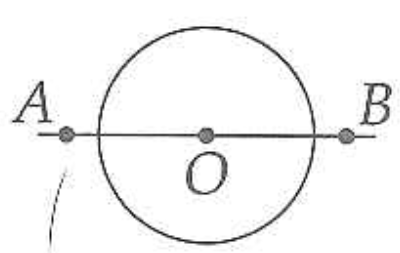
\includegraphics[width=0.3\linewidth]{Geometria/imgs/sol_aopsgeo_2_6}
		\caption{Solución de \ref{aopsg_p2_6}}
		\label{sol_aopsgeo_2_6}
	\end{figure}
\end{ejemplo}

\begin{ejemplo}
	\label{aopsg_p2_7}
	(2.7 de \cite{Aops_Geometria}). En la figura \ref{aopsgeo_p2_7} cuánto mide el ángulo $\angle WXY$?
	
	\begin{figure}[H]
		\centering
		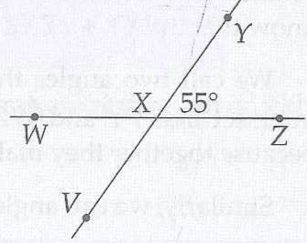
\includegraphics[width=0.6\linewidth]{Geometria/imgs/aopsgeo_p2_7}
		\caption{Ejemplo \ref{aopsg_p2_7}}
		\label{aopsgeo_p2_7}
	\end{figure}
	\textbf{Rta:} Como todo el ángulo $\angle WXZ = 180\degree $ entonces $\angle YXW = 180\degree - 55\degree = 125\degree $
	
\end{ejemplo}

\begin{ejemplo}
	\label{aopsg_p2_8}
	(2.8 de \cite{Aops_Geometria}). En la figura \ref{aopsgeo_p2_8}, si $\angle MPN=72\degree$, cuánto mide $\angle LPO$?
	
	\begin{figure}[H]
		\centering
		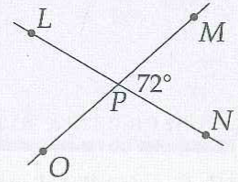
\includegraphics[width=0.6\linewidth]{Geometria/imgs/aopsgeo_p2_8}
		\caption{Ejemplo \ref{aopsg_p2_8}}
		\label{aopsgeo_p2_8}
	\end{figure}
	\textbf{Rta:} Como todo el ángulo $\angle NPL = 180\degree $ entonces $\angle MPL = 180\degree - 72\degree = 108\degree $. Y como $\angle MPO = 180\degree $ entonces $\angle LPO = 180\degree - 108\degree = 72\degree $.
\end{ejemplo}

\begin{ejemplo}
	\label{aopsg_p2_9}
	(2.9 de \cite{Aops_Geometria}). En la figura \ref{aopsgeo_p2_9}, probar que $\angle NPM = \angle LPO$.
	
	\begin{figure}[H]
		\centering
		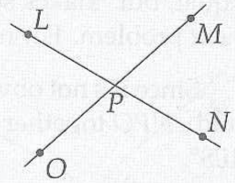
\includegraphics[width=0.6\linewidth]{Geometria/imgs/aopsgeo_p2_9}
		\caption{Ejemplo \ref{aopsg_p2_9}}
		\label{aopsgeo_p2_9}
	\end{figure}
	\textbf{Rta:} Si suponemos por ejemplo que $\angle MPN=72\degree$, como vimos en el ejercicio \ref{aopsg_p2_8} $\angle LPO = 72\degree $, es decir $\angle NPM = \angle LPO$. \textbf{Pero cuidado!} acá solo probamos un caso.
	\\
	\textbf{OJO. }En una prueba se deben probar todos los casos, un ejemplo no es una prueba
	\\
	Los ejemplos pueden servir como guía de como hacer la prueba, en este caso como $\overleftrightarrow{MPO}$ es una recta entonces $$\angle NPM = 180\degree - \angle OPN $$ y como $\overleftrightarrow{LPN}$ es una recta  entonces $$\angle LPO = 180\degree - \angle OPN$$. Entonces $$\angle NPM = \angle LPO$$.
\end{ejemplo}

\textbf{Importante: }Los \textbf{ángulos opuestos por un vértice} al intersectarse dos rectas son siempre iguales. Para representar ángulos iguales se usan marcas como las que se ven en la figura \ref{angulos_opuestos_iguales}.

\begin{figure}[H]
	\centering
	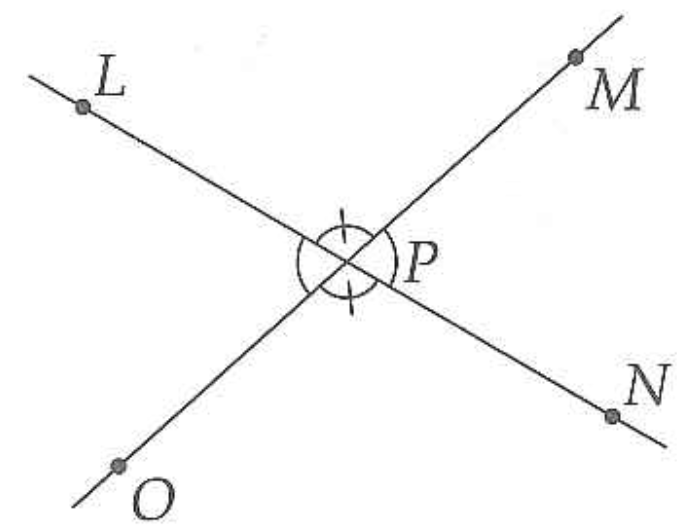
\includegraphics[width=0.5\linewidth]{Geometria/imgs/angulos_opuestos_iguales}
	\caption{Angulos opuestos por un vértice al intersectarse dos rectas son siempre iguales}
	\label{angulos_opuestos_iguales}
\end{figure}

\begin{itemize}
	\item Cuando dos ángulos forman juntos uno de $180\degree$ se llaman \textbf{ángulos suplementarios}. Ejemplo, el ángulo suplementario de $\angle ABC= 30\degree$ es el ángulo $\angle CBD = 150\degree $. Ver Figura \ref{suplementarios}
	
	\begin{figure}[H]
		\centering
		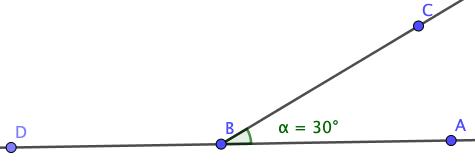
\includegraphics[width=0.7\linewidth]{Geometria/imgs/suplementarios}
		\caption{Ángulos \textbf{suplementarios} $\angle ABC$ y $\angle BCD$.}
		\label{suplementarios}
	\end{figure}
	
	\item Cuando dos ángulos forman juntos uno de $90\degree$ se llaman \textbf{ángulos complementarios}. Ejemplo, el ángulo suplementario de $\angle ABC= 40\degree$ es el ángulo $\angle CBD = 50\degree $. Ver Figura \ref{complemetarios}
	
	\begin{figure}[H]
		\centering
		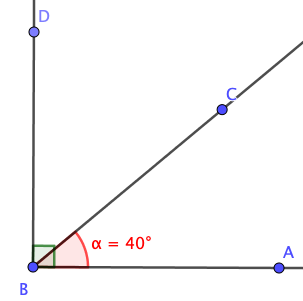
\includegraphics[width=0.5\linewidth]{Geometria/imgs/complementarios}
		\caption{Ángulos \textbf{complementarios} $\angle ABC$ y $\angle BCD$.}
		\label{complementarios}
	\end{figure}
	
	\item Cuando dos rectas se intersectan y forman un ángulo de $90\degree$ se llaman \textbf{rectas perpendiculares}. Ejemplo, en la figura \ref{rectasperpendiculares} las rectas $\overleftrightarrow{AB}$ y $\overleftrightarrow{CD}$ son perpendiculares, esto se denota $\overleftrightarrow{AB}\perp \overleftrightarrow{CD}$.
	
	\begin{figure}[H]
		\centering
		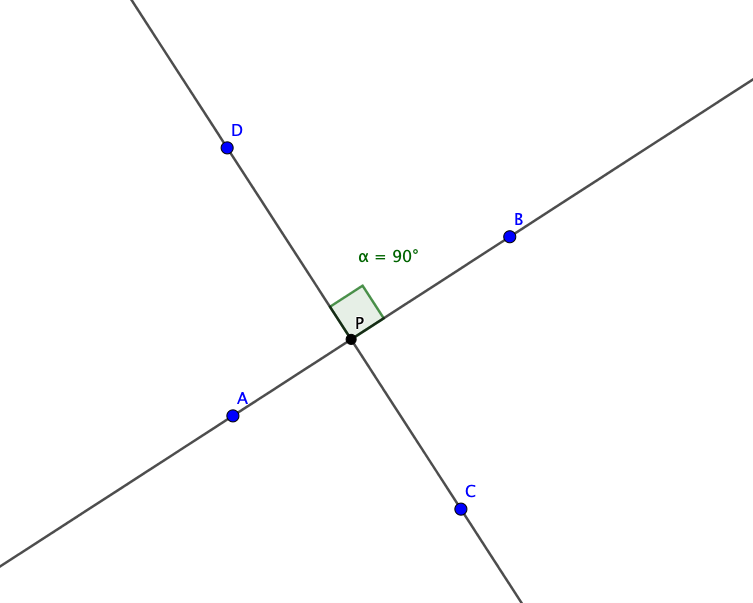
\includegraphics[width=0.5\linewidth]{Geometria/imgs/rectasperpendiculares}
		\caption{Las rectas $\protect \overleftrightarrow{AB}$ y $\protect\overleftrightarrow{CD}$ son perpendiculares, esto se denota $\protect\overleftrightarrow{AB}\protect\perp \protect\overleftrightarrow{CD}$.}
		\label{rectasperpendiculares}
	\end{figure}
	
\end{itemize}

\begin{ejemplo}
	La medida de un ángulo es igual a $\frac{5}{4}$ de la medida de su ángulo suplementario. Hacer un dibujo y calcular ambos ángulos.
	\textbf{Rta:} 
\end{ejemplo}

\begin{ejemplo} \label{ejemplo_ex2p68_udeageo}
	(Ex. 2 p68 de \cite{Udea_geometria}). En la figura \ref{ex2p68udeageo} las rectas $AC$ y $BD$ son dos rectas que se cortan en $O$ y $\angle AOD= 2\angle AOB$, hallar la medida de $\angle AOB, \angle BOC, \angle COD$ y $\angle DOA$.
	
	\begin{figure}[H]
		\centering
		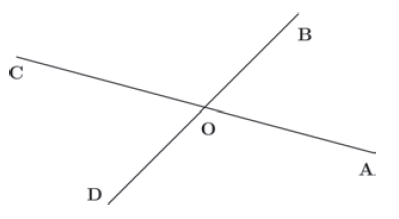
\includegraphics[width=0.5\linewidth]{Geometria/imgs/Ex2_p68_Udea_geo}
		\caption{Ejemplo de \ref{ejemplo_ex2p68_udeageo}}
		\label{ex2p68udeageo}
	\end{figure}
	\textbf{Rta:} 
\end{ejemplo}

\begin{ejemplo}\label{ejemplo_ej11_3_p76_udeageo}
	(Ej. 11.3 p.76 de \cite{Udea_geometria}).
	Si dos rectas distintas se cortan en un punto y uno de los ángulos que se forman mide $x\degree$, escribir en términos de $x$ la medida de los otros ángulos.
	\textbf{Rta:} 
\end{ejemplo}

\begin{ejemplo} \label{ejemplo_ej11_4_p76_udeageo}
	(Ej. 11.4 p.76 de \cite{Udea_geometria}). En la figura \ref{ex2p68udeageo} las rectas $AB,CD$ y $EF$ se cortan en $K$ y $\angle a= 2\angle c$, demostrar que $\angle b = \angle c$.
	
	\begin{figure}[H]
		\centering
		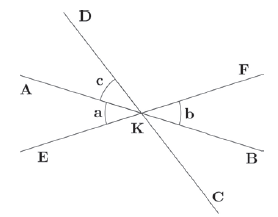
\includegraphics[width=0.5\linewidth]{Geometria/imgs/ej11_4_p76_udeageo}
		\caption{Ejemplo de \ref{ejemplo_ej11_4_p76_udeageo}}
		\label{ej11_4_p76_udeageo}
	\end{figure}
	\textbf{Rta:} 
\end{ejemplo}

\newpage
\begin{center}
	\vspace{-1cm}
	\subsubsection{Ejercicios: Angulos. Opuestos por el vértice, complementarios, suplementarios.} \label{ejercicios_subsection_opuestosvertices_complementarios_suplementarios}
\end{center}

\begin{enumerate}
	\item (Pag 191 de \cite{Dimensions_Math_7A}). Responda verdadero o falso:
	\begin{enumerate}[label=\Alph*) ]
		\item $31\degree$ y $71\degree$	son complementarios.
		\item $25\degree$ y $65\degree$	son complementarios.
		\item $128\degree$ y $62\degree$ son suplementarios.
		\item $40\degree$ y $140\degree$ son suplementarios.						
	\end{enumerate}
	
	\item (Pag 191 de \cite{Dimensions_Math_7A}). Responda las siguientes preguntas:
	\begin{enumerate}[label=\Alph*) ]
		\item Qué ángulo es complementario a $20\degree$ ?
		\item Qué ángulo es complementario a $42\degree$ ?
		\item Qué ángulo es suplementario a $43\degree$ ?
		\item Qué ángulo es suplementario a $76\degree$ ?
	\end{enumerate}	
	
	\item (Pag 191 de \cite{Dimensions_Math_7A}). En ambos ejercicios $AOB$ es una recta.
	\begin{enumerate}[label=\Alph*) ]
		\item \label{5aPAG91_dim7A}Encontrar cuánto mide $a$ en la figura \ref{dimensions_7A_p191_5a}.
		\begin{figure}[H]
			\centering
			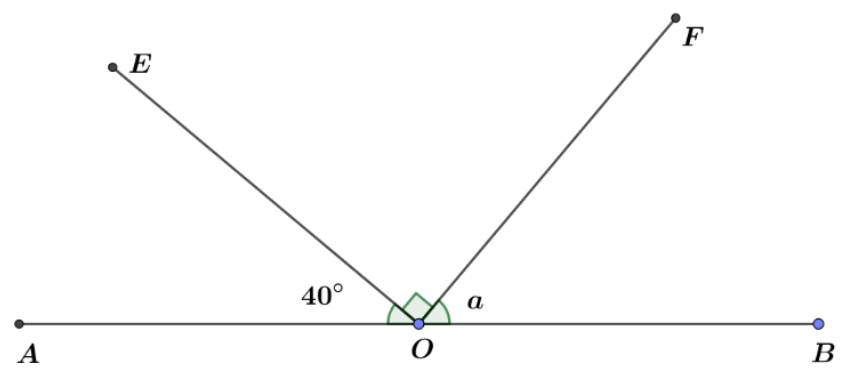
\includegraphics[width=0.6\linewidth]{Geometria/imgs/dimensions_7A_p191_5a}
			\caption{Ejercicio \ref{5aPAG91_dim7A}}
			\label{dimensions_7A_p191_5a}
		\end{figure}
		\item \label{5bPAG91_dim7A}Encontrar cuánto mide $b$ en la figura \ref{dimensions_7A_p191_5b}.
		\begin{figure}[H]
			\centering
			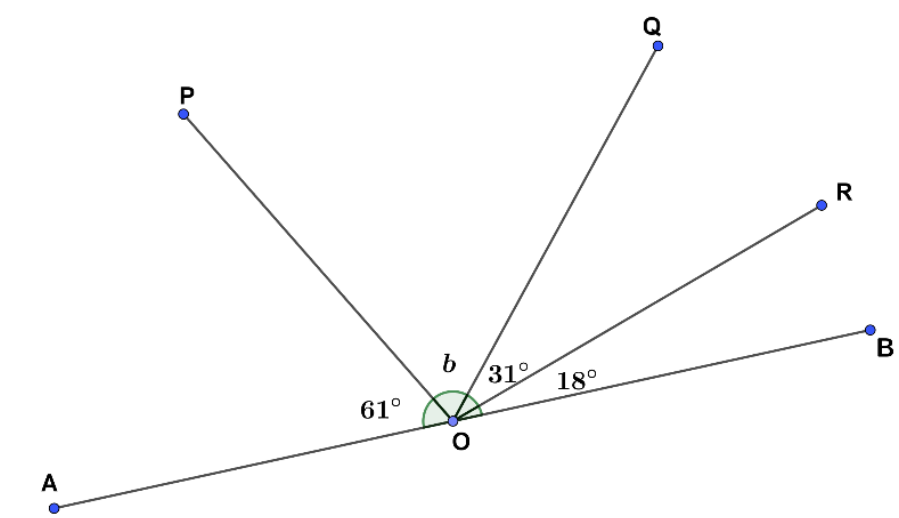
\includegraphics[width=0.6\linewidth]{Geometria/imgs/dimensions_7A_p191_5b}
			\caption{Ejercicio \ref{5bPAG91_dim7A}}
			\label{dimensions_7A_p191_5b}
		\end{figure}
	\end{enumerate}	
	
	\item (Pag 191 de \cite{Dimensions_Math_7A}). Responder ambos ejercicios:
	\begin{enumerate}[label=\Alph*) ]
		\item \label{6aPAG91_dim7A}Encontrar cuánto mide $x$ en la figura \ref{dimensions_7A_p191_6a}.
		\begin{figure}[H]
			\centering
			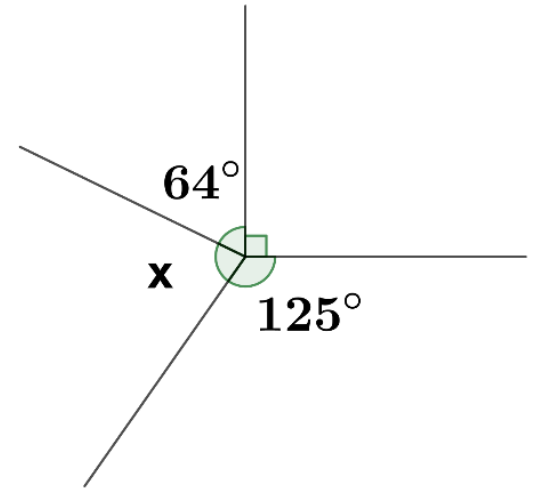
\includegraphics[width=0.3\linewidth]{Geometria/imgs/dimensions_7A_p191_6a}
			\caption{Ejercicio \ref{6aPAG91_dim7A}}
			\label{dimensions_7A_p191_6a}
		\end{figure}
		\item \label{6bPAG91_dim7A}Encontrar cuánto mide $x$ en la figura \ref{dimensions_7A_p191_6b}.
		\begin{figure}[H]
			\centering
			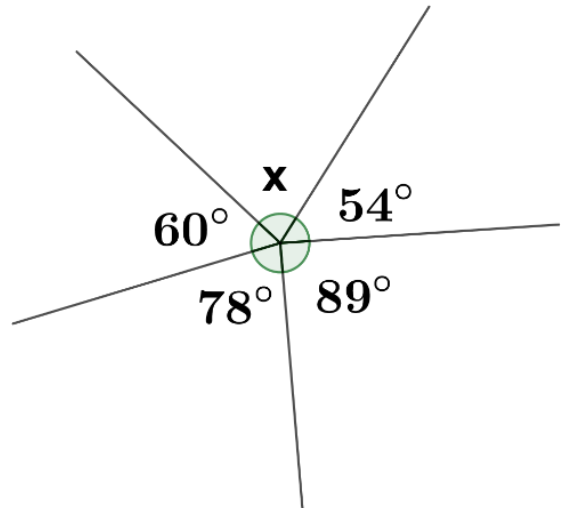
\includegraphics[width=0.3\linewidth]{Geometria/imgs/dimensions_7A_p191_6b}
			\caption{Ejercicio \ref{6bPAG91_dim7A}}
			\label{dimensions_7A_p191_6b}
		\end{figure}
	\end{enumerate}	
	
	\item (Pag 191 de \cite{Dimensions_Math_7A}). En ambos ejercicios, se intersectan las rectas $AB$ y $CD$. Encontrar la medida de los ángulos 
	\begin{enumerate}[label=\Alph*) ]
		\item \label{7aPAG91_dim7A} $x,y$ en la figura \ref{dimensions_7A_p191_7a}.
		\begin{figure}[H]
			\centering
			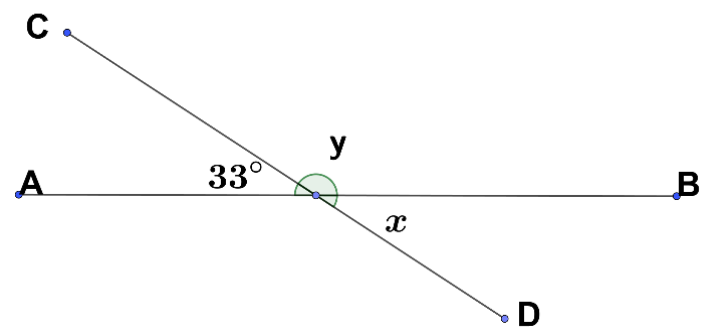
\includegraphics[width=0.35\linewidth]{Geometria/imgs/dimensions_7A_p191_7a}
			\caption{Ejercicio \ref{7aPAG91_dim7A}}
			\label{dimensions_7A_p191_7a}
		\end{figure}
		\item \label{7bPAG91_dim7A} $p,q$ en la figura \ref{dimensions_7A_p191_7b}.
		\begin{figure}[H]
			\centering
			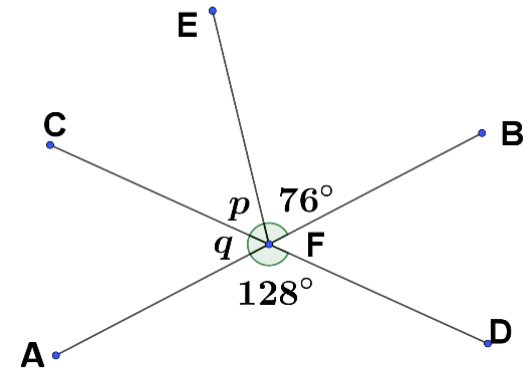
\includegraphics[width=0.35\linewidth]{Geometria/imgs/dimensions_7A_p191_7b}
			\caption{Ejercicio \ref{7bPAG91_dim7A}}
			\label{dimensions_7A_p191_7b}
		\end{figure}
	\end{enumerate}	
	
	\item \label{10PAG91_dim7A}(Pag 191 de \cite{Dimensions_Math_7A}). $A,B$ y $C$ están en la misma recta. Responder las siguientes preguntas en base a la figura \ref{dimensions_7A_p191_10}.
	\begin{enumerate}[label=\Alph*) ]
		\item Cuánto mide $x$?
		\item Qué tipo de ángulo es $\angle ABD$?
	\end{enumerate}	
	\begin{figure}[H]
		\centering
		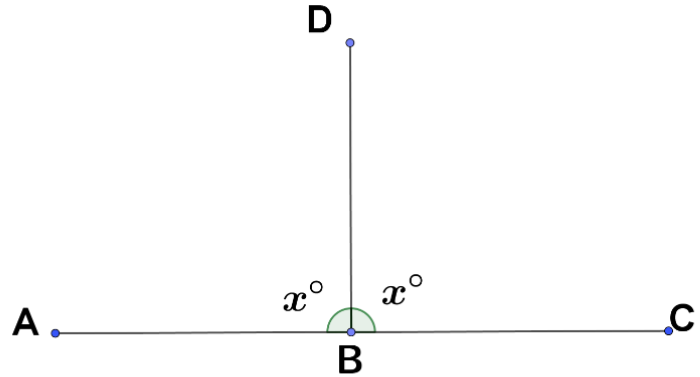
\includegraphics[width=0.35\linewidth]{Geometria/imgs/dimensions_7A_p191_10}
		\caption{Ejercicio \ref{10PAG91_dim7A}}
		\label{dimensions_7A_p191_10}
	\end{figure}
	
	\item \label{14aPAG91_dim7A}(Pag 191 de \cite{Dimensions_Math_7A}). En la figura \ref{dimensions_7A_p191_14a} encontrar el valor de $x$.	
	\begin{figure}[H]
		\centering
		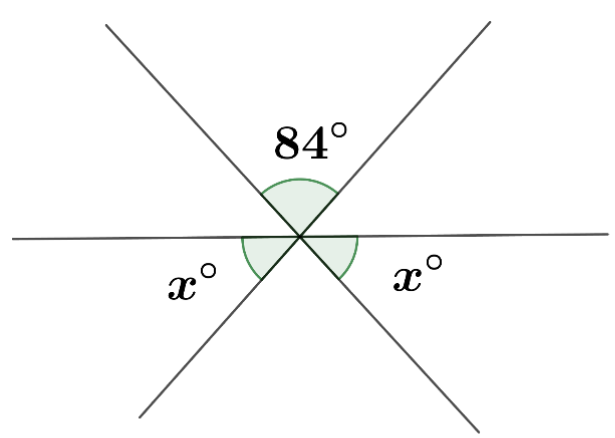
\includegraphics[width=0.35\linewidth]{Geometria/imgs/dimensions_7A_p191_14a}
		\caption{Ejercicio \ref{14aPAG91_dim7A}}
		\label{dimensions_7A_p191_14a}
	\end{figure}
	
	\item \label{8PAG91_dim7A}(Pag 191 de \cite{Dimensions_Math_7A}). 	Un ángulo desconocido cumple que su ángulo complementario es el doble que el, encontrar cuántos grados mide este ángulo.
	
	\item \label{9PAG91_dim7A}(Pag 191 de \cite{Dimensions_Math_7A}). 	Si los ángulos $2y\degree$ y $3y\degree$ son suplementarios, encontrar el valor de $y\degree$.
	
	\item \label{12PAG91_dim7A}(Pag 191 de \cite{Dimensions_Math_7A}). $P,Q$ y $R$ están en la misma recta. Responder las siguientes preguntas en base a la figura \ref{dimensions_7A_p191_12}.
	\begin{enumerate}[label=\Alph*) ]
		\item Cuánto mide $x$?
		\item Qué tipo de ángulo es $\angle SQT$?
	\end{enumerate}	
	\begin{figure}[H]
		\centering
		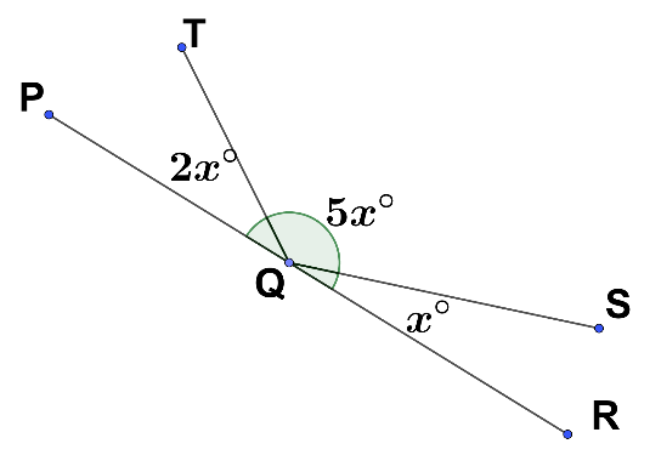
\includegraphics[width=0.35\linewidth]{Geometria/imgs/dimensions_7A_p191_12}
		\caption{Ejercicio \ref{12PAG91_dim7A}}
		\label{dimensions_7A_p191_12}
	\end{figure}
	\item \label{15PAG91_dim7A}(Pag 191 de \cite{Dimensions_Math_7A}). En la figura \ref{dimensions_7A_p191_15} $\overleftrightarrow{AB},\overleftrightarrow{BE}$ y $\overleftrightarrow{CF}$ se intersectan en $G$. Hallar los valores de $a,b$ y $c$.
	\begin{figure}[H]
		\centering
		\includegraphics[width=0.3\linewidth]{Geometria/imgs/dimensions_7A_p191_15}
		\caption{Ejercicio \ref{15PAG91_dim7A}}
		\label{dimensions_7A_p191_15}
	\end{figure}
	
	\item \label{clemenp152_1to4} (Pag. 152 de \cite{clemens}). En la figura \ref{figclemenp147_1to4},  $\angle EOC = 90\degree$ y las rectas $\overleftrightarrow{BE},\overleftrightarrow{CF},\overleftrightarrow{AD}$ se intersectan en el punto $O$. Responder las siguientes preguntas:
	\begin{enumerate}[label=\Alph*) ]
		\item Nombre todos los ángulos rectos que hay en la figura.
		\item Nombre los pares de ángulos rectos que sean opuestos por el vertice.
		\item Nombre los pares de ángulos agudos que sean opuestos por el vertice.
		\item Nombre los pares de ángulos obtusos que sean opuestos por el vertice.
		\item Nombre todos lod grupos de ángulos que sean iguales.							
	\end{enumerate}
	\begin{figure}[H]
		\centering
		\includegraphics[width=0.5\linewidth]{Geometria/imgs/clemenp147_1to4}
		\caption{Ejercicio \ref{clemenp152_1to4}}
		\label{figclemenp147_1to4}
	\end{figure}
	
	\item \label{clemenp152_5to8} (Pag. 152 de \cite{clemens}). En la figura \ref{figclemenp147_5to8},  $\angle 2 = 35\degree$. Complete las siguientes igualdades:
	\begin{enumerate}[label=\Alph*) ]
		\item $\angle 3 = $
		\item $\angle 1 = $
		\item $\angle 4 = $								
		\item $\angle 1 +\angle 4 = $			
	\end{enumerate}
	\begin{figure}[H]
		\centering
		\includegraphics[width=0.5\linewidth]{Geometria/imgs/clemenp147_5to8}
		\caption{Ejercicio \ref{clemenp152_1to4}}
		\label{figclemenp147_5to8}
	\end{figure}
	
	
	\item \label{P231_aopgeo} (2.3.1 de \cite{Aops_Geometria}). Encontrar $x,y$ y $z$ en la Figura \ref{ejer_P231_aopgeo}
	\begin{figure}[H]
		\centering
		\includegraphics[width=0.5\linewidth]{Geometria/imgs/aopsgeo_ejer_231}
		\caption{Ejercicio \ref{P231_aopgeo} }
		\label{ejer_P231_aopgeo}
	\end{figure}
	\item \label{P232_aopgeo} (2.3.2 de \cite{Aops_Geometria}).	Dibujar cada uno de los siguiente ángulos y encontrar la medida del ángulo que es \textbf{suplementario} a este:
	\begin{enumerate}[label=\Alph*) ]
		\item $\angle AOB = 120\degree$.
		\item $\angle COD = 45\degree$.
		\item $\angle EOF = 90\degree$.								
	\end{enumerate}
	
	\item \label{P233_aopgeo} (2.3.3 de \cite{Aops_Geometria}).	Dibujar cada uno de los siguiente ángulos y encontrar la medida del ángulo que es \textbf{complementario} a este:
	\begin{enumerate}[label=\Alph*) ]
		\item $\angle GOM = 30\degree$.
		\item $\angle IOJ = 45\degree$.
		\item $\angle KOL = 75\degree$.							
	\end{enumerate}
	
	\item \label{clemenp1471to6} (Pag. 148 de \cite{clemens}). En la figura \ref{figclemenp1471to6}, $\overleftrightarrow{AB} \perp \overrightarrow{OE}$ y $\angle 1 = \angle 2$. Responder las siguientes preguntas:
	\begin{enumerate}[label=\Alph*) ]
		\item Nombre un ángulo que sea suplementario a $\angle 1$.
		\item Nombre un ángulo que sea suplementario a $\angle COB$.
		\item Nombre un ángulo que sea complementario a $\angle COE $.
		\item Nombre un ángulo que sea complementario a $\angle 2$.	
		\item Por qué $\angle COE$ y $\angle DOE$ son iguales?
		\item Por qué $\angle COB$ y $\angle AOD$ son iguales?									
	\end{enumerate}
	\begin{figure}[H]
		\centering
		\includegraphics[width=0.5\linewidth]{Geometria/imgs/clemenp1471to6}
		\caption{Ejercicio \ref{clemenp1471to6}}
		\label{figclemenp1471to6}
	\end{figure}
	
	\item \label{clemenp1477to14} (Pag. 148 de \cite{clemens}). En la figura \ref{figclemenp147_7to14}, $\overleftrightarrow{AB} \perp \overleftrightarrow{EF}, \overleftrightarrow{CD} \perp \overleftrightarrow{HG}, \overleftrightarrow{AH} \perp \overleftrightarrow{HG}$ y $\overleftrightarrow{EG} \perp \overleftrightarrow{HG}$. Responder las siguientes preguntas:
	\begin{enumerate}[label=\Alph*) ]
		\item Nombre un ángulo que sea igual a $\angle COE$ y explique por qué es igual.
		\item Nombre un ángulo que sea igual a $\angle COA$ y explique por qué es igual.				
		\item Nombre dos ángulos que sean suplementarios a $\angle COE$.
		\item Nombre dos ángulos que sean complementarios a $\angle 3$.
		\item Nombre dos ángulos que sean complementarios a $\angle HOF$.
		\item Por qué $\angle COE$ y $\angle BOG$ son iguales?
		\item Por qué $\angle AOH$ y $\angle COE$ son iguales?	
		\item Por qué $\angle AOG$ y $\angle EOD$ son iguales?													
		\item Por qué $\angle 3$ y $\angle AOC$ son iguales?	
		\item Por qué $\angle 3$ y $\angle AOD$ son suplementarios?									
	\end{enumerate}
	\begin{figure}[H]
		\centering
		\includegraphics[width=0.7\linewidth]{Geometria/imgs/clemenp147_7to14}
		\caption{Ejercicio \ref{clemenp1477to14}}
		\label{figclemenp147_7to14}
	\end{figure}
	
	\item \label{clemenp147_15} (Pag. 148 de \cite{clemens}). Si un ángulo $\angle A = x$ entonces el ángulo complementario a $\angle A$ cuánto mide?
	\item \label{clemenp147_16} (Pag. 148 de \cite{clemens}). Si un ángulo $\angle B = x$ entonces el ángulo supplementario a $\angle B$ cuánto mide?	
	\item Dos ángulos son suplementarios. La medida de uno de ellos es cuatro veces la medida del otro. Encuéntrense las medidas de los dos ángulos.
	\item Dos ángulos son suplementarios. La medida de uno de ellos es $40\degree$ menos que el otro. Encuéntrense las medidas de los dos ángulos.		
	\item Dos ángulos son suplementarios. La medida de uno de ellos es $20\degree$ menos que tres veces (el triple) lamedida del otro. Encuéntrense las medidas de los dos ángulos.					
	
	\item \label{clemenp152_9to11} (Pag. 152 de \cite{clemens}). En la figura \ref{figclemenp147_9to11},  las rectas $\overleftrightarrow{RT}$ y $\overleftrightarrow{QS}$ se intersectan en el punto $V$. Responder las siguientes preguntas:
	\begin{enumerate}[label=\Alph*) ]
		\item Si $\angle RVQ = 4x$ y $\angle SVT = 2x+20$, entonces cuánto mide $\angle RVQ$?					
		\item Si $\angle QVT = 5x$ y $\angle RVS = 8x-45$, entonces cuánto mide $\angle RVS$?			
		\item Si $\angle RVQ = 2x+30$ y $\angle SVT = 3x+20$, entonces cuánto mide $\angle SVT$?			
	\end{enumerate}
	\begin{figure}[H]
		\centering
		\includegraphics[width=0.4\linewidth]{Geometria/imgs/clemenp147_9to11}
		\caption{Ejercicio \ref{clemenp152_9to11}}
		\label{figclemenp147_9to11}
	\end{figure}
	
	\item \label{clemenp165_} (Pag. 165 de \cite{clemens}). Diga si lo siguiente es verdadero o falso: " Si dos ángulos son suplementarios y son iguales, entonces ambos son rectos ``. Por qué?
	
	\item \label{udea_ejem10_5} (Ejemplo 10.5 de \cite{Udea_geometria}). En la figura \ref{udeaejemplo105},  $\angle PAM$ y $\angle 	MAJ$ son complementarios, y $\angle JAK$ y $MAJ$ también lo son. Probar que $\angle PAM = \angle JAK$.
	\begin{figure}[H]
		\centering
		\includegraphics[width=0.4\linewidth]{Geometria/imgs/udea_ejemplo_10_5}
		\caption{Ejercicio \ref{udea_ejem10_5}.}
		\label{udeaejemplo105}
	\end{figure}
	
\end{enumerate}

\newpage

\subsection{Ángulos entre paralelas.}\label{subsection_angulos_entre_paralelas}
Si tenemos un punto $A$ y una recta $l$, la \textbf{distancia del punto a la recta} es la longitud del segmento $AB$, donde $B$ es el punto de intersección de $l$ y una recta perpendicular $k$ que pasa por $A$. 

Recordemos que si tenemos una recta, podemos construir una recta que no la corte en ningún punto, esta es una \textbf{recta paralela}.  

\begin{itemize}
	\item Si $m$ es una recta y $k$ es paralela a $m$ esto lo denotamos como $m\parallel k$.
	\begin{figure}[H]
		\centering
		\includegraphics[width=0.7\linewidth]{Geometria/imgs/paralelas}
		\caption{}
		\label{paralelas_con_notacion}
	\end{figure}
	\item Si tengo una recta $m$ cuántas rectas paralelas hay a $m$?
	\item Si tengo una recta $r$ y $r\parallel s$, todos los puntos que están en $s$ tienen una propiedad en común, cuál crees que es? \textbf{Rta: }Todos están a la misma distancia de $r$.
\end{itemize}

\begin{exer}
	Construir una recta $l$ y a partir de ella contruir después una recta $n$ tal que $l\parallel n$ y estén separadas $5cm$. 
	\begin{itemize}
		\item Solo hay una recta paralela a $l$ que esté a $5cm$?
	\end{itemize}
\end{exer}

Si tenemos ahora que $r\parallel s$ y construimos una recta $t$ tal que $t\parallel s$
\begin{itemize}
	\item Será que $r\parallel t$?
	\item Las tres rectas son paralelas?
\end{itemize}

Si ahora construimos a $t$ de forma que no sea paralela, es decir, sea una secante.
\begin{itemize}
	\item Que observa? Que nuevas estructuras geométricas se forman?
	\item Mide todos los ángulos que se forman.
	\item Toma ahora otra recta secante y vuelve a medir los ángulos.
	\item A partir de la figura \ref{paralelas_angulos_iguales}, marca los ángulos que son iguales, con color y marcas.
	\begin{figure}[H]
		\centering
		\includegraphics[width=0.7\linewidth]{Geometria/imgs/paralelas_angulos_iguales}
		\caption{Viendo los ángulos iguales al cortar dos rectas paralelas.}
		\label{paralelas_angulos_iguales}
	\end{figure}
	\item Nombra los ángulos que son iguales en la figura \ref{paralelas_angulos_iguales}.
\end{itemize}

\begin{theorem} \textbf{(Ángulos en paralelas)}
	Si $r$ y $s$ son dos rectas paralelas (es decir $r\parallel s$) que son cortadas por una recta $t$ como se muestra en la figura \ref{paralelas_angulos_iguales_marca_color}, entonces se cumple que
	\[
	\color{red} \angle HJE =  \angle DJK = \angle FKN = \angle JKG,
	\]
	y 
	\[
	\color{blue}\angle HJD =  \angle EJK = \angle GKN = \angle JKF.
	\]
	
	\begin{figure}[H]
		\centering
		\includegraphics[width=0.7\linewidth]{Geometria/imgs/paralelas_angulos_iguales_marca_color}
		\caption{}
		\label{paralelas_angulos_iguales_marca_color}
	\end{figure}
\end{theorem}

\begin{ejemplo}{\ \\}
	\label{p2_11_aops_geo} (2.11 de \cite{Aops_Geometria})En la figura \ref{aopsgeo_2_11_pag25} $m\parallel n$ y conocemos la medida de un ángulo. Encontrar los valores de $a,b,c,w,x,y,z$.
	\begin{figure}[H]
		\centering
		\includegraphics[width=0.4\linewidth]{Geometria/imgs/aopsgeo_2_11_pag25}
		\caption{Ejemplo \ref{p2_11_aops_geo}.}
		\label{aopsgeo_2_11_pag25}
	\end{figure}
\end{ejemplo}

\begin{ejemplo}{\ \\}
	\label{ejemplo_problema_paralela_triangulo} En la figura \ref{problema_paralela_triangulo} $DEFG$ es un cuadrado y conocemos la medida de un ángulo. Encontrar la medida del ángulo $\angle JIE$. (Marcar la mayor cantidad de ángulos que puedas hallar)
	
	\begin{figure}[H]
		\centering
		\includegraphics[width=0.6\linewidth]{Geometria/imgs/problema_paralela_triangulo}
		\caption{Ejemplo \ref{ejemplo_problema_paralela_triangulo}.}
		\label{problema_paralela_triangulo}
	\end{figure}
\end{ejemplo}

\begin{exer}{\ \\}
	Crear un problema donde sea necesario usar ángulos y la propiedad de los ángulos en las rectas paralelas.
\end{exer}

\begin{itemize}
	\item Construyamos ahora una recta $f$ que pasa por los puntos $A$ y $B$ y una recta $s$ que se intersecta con $f$ en el punto $C$ formando un ángulo de $50\degree$ (Se puede usar la \textit{herramienta ángulo dado} en geogebra) como en la figura \ref{recta_y_secante_a_50_grados}
	\begin{figure}[H]
		\centering
		\includegraphics[width=0.6\linewidth]{Geometria/imgs/recta_y_secante_a_50_grados}
		%\caption{Ejemplo \ref{ejemplo_problema_paralela_triangulo}.}
		\label{recta_y_secante_a_50_grados}
	\end{figure}
	\item Si construimos una recta $l$ que pase por $H$ y que forme un ángulo de $50\degree $ con $s$, que puede decir sobre $l$ y $s$? \textbf{Rta: } Son paralelas.
	\begin{figure}[H]
		\centering
		\includegraphics[width=0.6\linewidth]{Geometria/imgs/si_angulos_entonces_son_paralelas}
		\label{si_angulos_entonces_son_paralelas}
	\end{figure}			
	\item Si hacemos lo mismo pero con otro ángulo será que siempre se cumple? (Usar la \textit{herramienta deslizador} en geogebra).
\end{itemize}


\begin{theorem} \textbf{(Paralelas conociendo los ángulos)}
	Si se cumple que
	\[
	\color{red} \angle HJE =  \angle DJK = \angle FKN = \angle JKG,
	\]
	y 
	\[
	\color{blue}\angle HJD =  \angle EJK = \angle GKN = \angle JKF.
	\]
	Entonces $r$ y $s$ son dos rectas paralelas (es decir $r\parallel s$)  \ref{paralelas_angulos_iguales_marca_color_2}, entonces 
	
	\begin{figure}[H]
		\centering
		\includegraphics[width=0.7\linewidth]{Geometria/imgs/paralelas_angulos_iguales_marca_color}
		\caption{}
		\label{paralelas_angulos_iguales_marca_color_2}
	\end{figure}
\end{theorem}

\begin{ejemplo}{\ \\}
	\label{ejer1_p176_clemens} (Ejercicio 1 pag 176 de \cite{clemens}) En la figura \ref{problema_paralela_triangulo}, las rectas fueron hechas por un joven que las copió de un libro, el joven las dibujó un poco torcidas pero anotó cómo estaba nombrado cada ángulo. El sabía también las siguientes propiedades, en base a cada una responder que par de rectas del dibujo son paralelas:
	\begin{enumerate}[label=\Alph*) ]
		\item $\angle 1 = \angle 9$.
		\item $\angle 3 = \angle 6$.
		\item $\angle 8 + \angle 10 = 180\degree$.
		\item $\angle 4 = \angle 9$.	
		\item $\angle 8 = \angle 12$.			
		\item $\angle 1 = \angle 8$.
	\end{enumerate}
	
	\begin{figure}[H]
		\centering
		\includegraphics[width=0.6\linewidth]{Geometria/imgs/clemens_pag176_ejer1}
		\caption{Ejemplo \ref{ejer1_p176_clemens}.}
		\label{clemens_pag176_ejer1}
	\end{figure}
\end{ejemplo}

\begin{ejemplo}
	\item  En la figura \ref{ejemplo_algebraico_angulos} se sabe que $p\parallel q$, $\angle 1 =3x+17$ y $\angle 4 = 9x-7$. Encontrar cuánto mide $\angle 1$ y $\angle 2$?
	\begin{figure}[H]
		\centering
		\includegraphics[width=0.4\linewidth]{Geometria/imgs/clemens187_24to25}
		\label{ejemplo_algebraico_angulos}
	\end{figure}
\end{ejemplo}

\begin{ejemplo}{\ \\}
	\label{ejem_2_12_aopsgeo} (2.12 de \cite{Aops_Geometria}) En la figura \ref{2_12_aopsgeo} se tiene que $\overleftrightarrow{AB}\parallel \overleftrightarrow{CD}$ y $\overleftrightarrow{AD}\parallel \overleftrightarrow{BC}$. También se conoce la medida de cuatro ángulos en términos de $x$ e $y$. Encontrar cuánto mide $x$ e $y$.
	\begin{figure}[H]
		\centering
		\includegraphics[width=0.6\linewidth]{Geometria/imgs/2_12_aopsgeo}
		\caption{Ejemplo \ref{ejem_2_12_aopsgeo}.}
		\label{2_12_aopsgeo}
	\end{figure}
\end{ejemplo}

\begin{ejemplo}{\ \\}
	\label{ejem_2_13_aopsgeo} (2.13 de \cite{Aops_Geometria}) En la figura \ref{2_13_aopsgeo} encontrar cuánto mide $x$.
	\begin{figure}[H]
		\centering
		\includegraphics[width=0.5\linewidth]{Geometria/imgs/2_13_aopsgeo}
		\caption{Ejemplo \ref{ejem_2_13_aopsgeo}.}
		\label{2_13_aopsgeo}
	\end{figure}
\end{ejemplo}

\begin{ejemplo}{\ \\}
	\label{ejem_2_14_aopsgeo} (2.14 de \cite{Aops_Geometria}) En la figura \ref{2_14_aopsgeo} encontrar cuánto mide $x$.
	\begin{figure}[H]
		\centering
		\includegraphics[width=0.4\linewidth]{Geometria/imgs/2_14_aopsgeo}
		\caption{Ejemplo \ref{ejem_2_14_aopsgeo}.}
		\label{2_14_aopsgeo}
	\end{figure}
\end{ejemplo}


\newpage
\begin{center}
	\vspace{-1cm}
	\subsubsection{Ejercicios: Ángulos entre paralelas.} \label{ejercicios_en_paralelas}
\end{center}

\begin{enumerate}
	\item \label{ejercicio_clemens176_2}(pag 176 ejercicio 2 de \cite{clemens}). El dibujo de la figura \ref{clemens176_2} está bien dibujado pero hay ciertos errores en las medidas de los ángulos. Haga una lista de todas las contradicciones que note en la figura.
	\begin{figure}[H]
		\centering
		\includegraphics[width=0.5\linewidth]{Geometria/imgs/clemens176_2}
		\caption{Ejercicio \ref{ejercicio_clemens176_2}}
		\label{clemens176_2}
	\end{figure}
	
	\item \label{ejercicio_clemens176_3}(pag 176 ejercicio 3 de \cite{clemens}). Mencione 4 formas diferentes de poder probar que dos rectas son paralelas (Hacer dibujo si lo ve neesario).
	
	\item  \label{ejercicio_clemens176_6} (pag 176 ejercicio 6 de \cite{clemens}). Qué pares de ángulos de la figura \ref{clemens176_6} se podría probar que son iguales para mostrar que $\overleftrightarrow{AB}\parallel \overleftrightarrow{CD}$?
	\begin{figure}[H]
		\centering
		\includegraphics[width=0.5\linewidth]{Geometria/imgs/clemens176_6}
		\caption{Ejercicio \ref{ejercicio_clemens176_6}}
		\label{clemens176_6}
	\end{figure}
	
	\item \label{ejercicio_clemens176_7} (pag 176 ejercicio 7 de \cite{clemens}). Qué pares de ángulos de la figura \ref{clemens176_6} se podría probar que son suplementarios para concluir que $\overleftrightarrow{AB}\parallel \overleftrightarrow{CD}$?
	
	\item  \label{ejercicio_clemens178_16} (pag 178 ejercicio 16 de \cite{clemens}). En la figura \ref{clemens178_16} se sabe que $AB\perp BC$, $DC\perp BC$ y $\angle 1 = \angle 4$. Mostrar que $\overleftrightarrow{BF}\parallel \overleftrightarrow{GC}$?
	\begin{figure}[H]
		\centering
		\includegraphics[width=0.5\linewidth]{Geometria/imgs/clemens178_16}
		\caption{Ejercicio \ref{ejercicio_clemens178_16}}
		\label{clemens178_16}
	\end{figure}
	
	\item  \label{ejercicio_clemens178_19} (pag 178 ejercicio 19 de \cite{clemens}). En la figura \ref{clemens178_19} se sabe que $\angle 4 y \angle 5$ y $\angle 2 + \angle 3 + \angle 5 = 180\degree  $. Mostrar que $AB\parallel CD$?
	\begin{figure}[H]
		\centering
		\includegraphics[width=0.5\linewidth]{Geometria/imgs/clemens178_19}
		\caption{Ejercicio \ref{ejercicio_clemens178_19}}
		\label{clemens178_19}
	\end{figure}
	
	\item  \label{ejercicio_clemens183_6} (pag 183 ejercicio 6 de \cite{clemens}). En la figura \ref{clemens183_6} se sabe que $\angle 1 =  \angle 2$ y $\angle 3 =\angle 4 $. Mostrar que $p\parallel r$?
	\begin{figure}[H]
		\centering
		\includegraphics[width=0.5\linewidth]{Geometria/imgs/clemens183_6}
		\caption{Ejercicio \ref{ejercicio_clemens183_6}}
		\label{clemens183_6}
	\end{figure}
	
	\item  \label{ejercicio_clemens183_7} (pag 183 ejercicio 7 de \cite{clemens}). En la figura \ref{clemens183_7} se sabe que $\angle 1 + \angle 2 =180\degree$ y $\angle 3 +\angle 4 =180\degree $. Mostrar que $p\parallel r$?
	\begin{figure}[H]
		\centering
		\includegraphics[width=0.5\linewidth]{Geometria/imgs/clemens183_7}
		\caption{Ejercicio \ref{ejercicio_clemens183_7}}
		\label{clemens183_7}
	\end{figure}
	
	\item  \label{ejercicio_clemens186_1to7} (pag 186 ejercicio 1-7 de \cite{clemens}). En la figura \ref{clemens186_1to7} se sabe que $p\parallel q$ y  $\angle 3 = 53\degree$. Encontrar la medida de los ángulos $\angle 1, \angle 2, \angle 4, \angle 5, \angle 6, \angle 7, \angle 8$.
	\begin{figure}[H]
		\centering
		\includegraphics[width=0.5\linewidth]{Geometria/imgs/clemens186_1to7}
		\caption{Ejercicio \ref{ejercicio_clemens186_1to7}}
		\label{clemens186_1to7}
	\end{figure}
	
	\item  \label{ejercicio_clemens186_8to12} (pag 186 ejercicio 8-12 de \cite{clemens}). En la figura \ref{clemens186_8to12} se sabe que $p\parallel q$, $\angle 1 = 125\degree$ y $\angle 4 = 143\degree$. Encontrar la medida de los ángulos $\angle 2, \angle 3, \angle 5, \angle 7, \angle 6$.
	\begin{figure}[H]
		\centering
		\includegraphics[width=0.5\linewidth]{Geometria/imgs/clemens186_8to12}
		\caption{Ejercicio \ref{ejercicio_clemens186_8to12}}
		\label{clemens186_8to12}
	\end{figure}
	
	\item  \label{ejercicio_clemens186_13to22} (pag 186 ejercicio 13-22 de \cite{clemens}). En la figura \ref{clemens186_13to22} se sabe que $\overleftrightarrow{AB} \parallel \overleftrightarrow{CD}$, $\overleftrightarrow{AD} \parallel \overleftrightarrow{BC}$, además $\angle ADC= 110\degree$ y $\angle ACD= 28\degree$. Encontrar la medida de los ángulos $\angle 1, \angle 2, \angle 3, \angle 4, \angle 5, \angle 6$, $ \angle 9, \angle 10, \angle BCD, \angle BAD$.
	\begin{figure}[H]
		\centering
		\includegraphics[width=0.5\linewidth]{Geometria/imgs/clemens186_13to22}
		\caption{Ejercicio \ref{ejercicio_clemens186_13to22}}
		\label{clemens186_13to22}
	\end{figure}
	
	\item  \label{ejercicio_clemens186_23} (pag 186 ejercicio 23 de \cite{clemens}). En la figura \ref{clemens186_23} se sabe que $\angle BCD =70\degree$. Cuánto deben medir los ángulos $\angle ABC, \angle CDA$ y $\angle DAB$ para que $\overleftrightarrow{AB} \parallel \overleftrightarrow{CD}$ y  $\overleftrightarrow{AD} \parallel \overleftrightarrow{BC}$?
	\begin{figure}[H]
		\centering
		\includegraphics[width=0.4\linewidth]{Geometria/imgs/clemens186_23}
		\caption{Ejercicio \ref{ejercicio_clemens186_23}}
		\label{clemens186_23}
	\end{figure}
	
	\item  \label{ejercicio_clemens187_24to25} (pag 187 ejercicio 24 de \cite{clemens}). En la figura \ref{clemens187_24to25} se sabe que $p\parallel q$, $\angle 1 =2x+3$ y $\angle 4 = 7x-12$. Encontrar cuánto mide $\angle 1$ y $\angle 2$?
	\begin{figure}[H]
		\centering
		\includegraphics[width=0.4\linewidth]{Geometria/imgs/clemens187_24to25}
		\caption{Ejercicios \ref{ejercicio_clemens187_24to25} y \ref{ejercicio_clemens187_24}.}
		\label{clemens187_24to25}
	\end{figure}
	
	\item  \label{ejercicio_clemens187_24} (pag 187 ejercicio 25 de \cite{clemens}). En la figura \ref{clemens187_24to25} sabemos que $p\parallel q$, pero ahora se tiene que $\angle 1 =2x+4$, $\angle 5= 3y+6$ y $\angle 2 = 4y+6$. Encontrar cuánto mide $\angle 1,\angle 2$ y $\angle 5$?
	
	\item  \label{ejercicio_clemens187_31} (pag 187 ejercicio 31 de \cite{clemens}). En la figura \ref{clemens187_31} se sabe que $p\parallel q$ y $s\parallel t$. Probar que $\angle 1 = \angle 7$ y $\angle 2 = \angle 9$.
	\begin{figure}[H]
		\centering
		\includegraphics[width=0.4\linewidth]{Geometria/imgs/clemens187_31}
		\caption{Ejercicio \ref{ejercicio_clemens187_31}}
		\label{clemens187_31}
	\end{figure}
	
	\item  \label{ejercicio_aopsgeo_2_4_1} (2.4.1 de \cite{Aops_Geometria}). En la figura \ref{aopsgeo_2_4_1} hallar el valor de $x$ e $y$.
	\begin{figure}[H]
		\centering
		\includegraphics[width=0.4\linewidth]{Geometria/imgs/aopsgeo_2_4_1}
		\caption{Ejercicio \ref{ejercicio_aopsgeo_2_4_1}}
		\label{aopsgeo_2_4_1}
	\end{figure}
	
	\item  \label{ejercicio_aopsgeo_2_4_2} (2.4.2 de \cite{Aops_Geometria}). En la figura \ref{aopsgeo_2_4_2} probar que $\angle A =\angle C$ y $\angle B = \angle C$.
	\begin{figure}[H]
		\centering
		\includegraphics[width=0.4\linewidth]{Geometria/imgs/aopsgeo_2_4_2}
		\caption{Ejercicio \ref{ejercicio_aopsgeo_2_4_2}}
		\label{aopsgeo_2_4_2}
	\end{figure}
	
	\item  \label{ejercicio_aopsgeo_2_4_3} (2.4.3 de \cite{Aops_Geometria}). En la figura \ref{aopsgeo_2_4_3} hallar el valor de $x$.
	\begin{figure}[H]
		\centering
		\includegraphics[width=0.4\linewidth]{Geometria/imgs/aopsgeo_2_4_3}
		\caption{Ejercicio \ref{ejercicio_aopsgeo_2_4_3}}
		\label{aopsgeo_2_4_3}
	\end{figure}
	
	\item  \label{ejercicio_aopsgeo_2_4_4} (2.4.4 de \cite{Aops_Geometria}). En la figura \ref{aopsgeo_2_4_4} hallar el valor de $x$.
	\begin{figure}[H]
		\centering
		\includegraphics[width=0.4\linewidth]{Geometria/imgs/aopsgeo_2_4_4}
		\caption{Ejercicio \ref{ejercicio_aopsgeo_2_4_4}}
		\label{aopsgeo_2_4_4}
	\end{figure}
	
	\item  \label{ejercicio_aopsgeo_2_4_5} (2.4.5 de \cite{Aops_Geometria}). En la figura \ref{aopsgeo_2_4_5} hallar el valor de $x$ e $y$.
	\begin{figure}[H]
		\centering
		\includegraphics[width=0.4\linewidth]{Geometria/imgs/aopsgeo_2_4_5}
		\caption{Ejercicio \ref{ejercicio_aopsgeo_2_4_5}}
		\label{aopsgeo_2_4_5}
	\end{figure}
	
\end{enumerate}
\newpage	

\chapter{Congruencia}\label{seccioncongruncias}

\subsection*{Actividad de construcción de triángulos únicos}\label{sub.sec.construccion.de.triangulos.unicos}
Para esta actividad será necesario:

\begin{itemize}
	\item Papel.
	\item Tijeras.
	\item Transportador.
	\item Compás.
\end{itemize}

%Diremos que un triángulo es \textbf{único} cuando sin importar giros o rotaciones
\begin{enumerate}
	\item Dibujar uno o más triángulo cuyos lados midan 5 cm, 7 cm y 10 cm.
	\begin{enumerate}
		\item Comparar los triángulos con los de sus compañeros. ¿Que observan?
	\end{enumerate}
	\textit{Concluir: Son el mismo}
	\item Utilizar un segmento de 5 cm, otro de 7 cm y un ángulo de $50\degree$ para construir uno o más triángulos. 
	\begin{enumerate}
		\item Comparar los triángulos con los de sus compañeros. ¿Que observan?
		\item ¿Dónde debe ir el ángulo para poder construir triángulos únicos?
	\end{enumerate}
	\textit{Concluir: Debe ir en medio de los lados para poder construir un único triángulo.}
	\item Utilizar un segmento de  7 cm, un ángulo de $50\degree$ y otro de $60\degree$ para construir uno o más triángulos. 
	\begin{enumerate}
		\item Comparar los triángulos con los de sus compañeros. ¿Que observan?
		\item ¿Dónde debe ir el lado para poder construir triángulos únicos?
	\end{enumerate}
	\textit{Concluir: Debe ir en medio de los ángulos para poder construir un único triángulo.}
	\item Utilizar un ángulo de $40\degree$, otro de $60\degree$ y un tercero de $80\degree$ para construir uno o más triángulos. 
	\begin{enumerate}
		\item ¿Es posible formar con esto un único triángulo?
	\end{enumerate}
	\textit{Concluir: No, se pueden generar muchos triángulo diferentes.}
	\item Usar los siguientes tríos de medidas para construir triángulos.
	\begin{itemize}
		\item 3 cm, 4 cm, 10 cm.
		\item 2 cm, 6 cm, 5 cm.
		\item 12 cm, 6 cm, 6 cm.
		\item 7 cm, 4 cm, 8 cm.
	\end{itemize}
	\begin{enumerate}
		\item ¿Qué observa? ¿Pudo construir los triángulos?
		\item Compare la medida de dos lados con la del tercero. ¿Que relación hay?
	\end{enumerate}
	\textit{Concluir: la suma de ellos es mayor que la medida del tercer lado}
	
	\item \underline{Cierre de actividad}
	\begin{enumerate}
		\item ¿Cuáles condiciones deben darse para formar un único triángulo?
		\begin{itemize}
			\item ¿La medida de los 3 lados?
			\item ¿La medida de 2 lados y el ángulo entre ellos?
			\item ¿La medida de 2 lados y un ángulo que no esté entre ellos?
			\item ¿2 ángulos y un lado?
			\item ¿3 ángulos?
		\end{itemize}
		\item ¿Que relación hay entre las medidas de los lados de un triángulo?
		
		\textit{Solución: A esto se le llama \textbf{Desigualdad Triangular}. La suma de cualesquiera dos lados del triángulo, debe ser mayor que la del tercero.}
	\end{enumerate}
	
	
\end{enumerate}
\section{Definiciones básicas.}\label{definiciones.basicas.congruencias}
Ver las siguientes figuras:

\begin{figure}[H]
	\centering
	\includegraphics[width=0.5\textwidth]{Geometria/imgs/congruencia_piso.jpg} 
	\caption{Piso 1}
	\label{congurncia.figura.1}
\end{figure}

\begin{figure}[H]
	\centering
	\includegraphics[width=0.5\textwidth]{Geometria/imgs/congruencia_piso_2.JPG}
	\caption{Piso 2}
	\label{congurncia.figura.2}
\end{figure}

\begin{figure}[H]
	\centering
	\includegraphics[width=0.5\textwidth]{Geometria/imgs/congruencia_piso_3.jpg}
	\caption{Piso 3}
	\label{congurncia.figura.3}
\end{figure}

\begin{figure}[H]
	\centering
	\includegraphics[width=0.5\textwidth]{Geometria/imgs/congruencia_piso_4.jpg}
	\caption{Piso 4}
	\label{congurncia.figura.4}
\end{figure}

Se ve que estos pisos están formados por figuras iguales, es ahí cuando se dice que estas figuras son \textbf{congruentes.}

\section*{Actividad de fuguras congruentes}\label{activ.construccion.figuras.congruentes}
Para esta actividad será necesario:

\begin{itemize}
	\item Papel.
	\item Tijeras.
	\item Papel calcante.
	\item Colores.
	
\end{itemize}

\begin{enumerate}
	\item Trazar un triángulo $ABC$ cualquiera en una hoja. Luego calcarlo y nombrar al nuevo triangulo $DEF$.
	\item Marcar con el mismo estilo los ángulo correspondientemente iguales.
	
	\textit{Observación.} Observe que de $\triangle ABC$ y $\triangle DEF$ podemos concluir que:
	\begin{itemize}
		\item $AB=DE,\; BC=EF,\; CA=FD$.
		\item $\angle CAB = \angle FDE,\; \angle ABC = \angle DEF,\; \angle BCA = \angle EFD,\; $
	\end{itemize}
	
	Entonces decimos que estos triángulo son congruentes. Esto se escribe como $$\triangle ABC \cong \triangle DEF.$$
	\item \textbf{Ojo.} Es importante el orden en que se escriben los vértices. Pues $$\triangle ABC \not \cong \triangle FED.$$
\end{enumerate}

\begin{defi}
	Dos figuras son \textbf{Congruentes} si:
	\begin{itemize}
		\item Todos los lados correspondientes son iguales.
		\item Todos los ángulos correspondientes son iguales.
	\end{itemize}
\end{defi}

Ver las siguientes figuras y plantear su congruencia:

\begin{figure}[H]
	\centering
	\includegraphics[width=0.8\textwidth]{Geometria/imgs/DEFI CONGRUENTES EJEMPLO1.JPG}
	\caption{Triangulos 1}
	\label{defi.congruencia.fig1}
\end{figure}
